% !TEX encoding = UTF-8 Unicode
%!TEX TS-program = xelatex

\chapter{基于三维带液贮箱模型的POGO稳定性分析}

\section{带液贮箱的建模方法}
\label{sec:3D-Liquid-Tank-Modelling}
为了证明引入带液贮箱三维模型的必要性,本节将首先对于传统简化贮箱模型进行简要介绍。通过公式推导和理论分析,指出了该方法在液体建模方面引入了过多理想假设,从而不再适用于对模型精度要求较高的POGO稳定性分析。接下来,针对带液贮箱的三维模型建立,文章分别就贮箱内液体建模和贮箱壳体建模两方面进行了详细说明。最后,通过对比两种方法的系统固有频率算例结果,指出了带液贮箱三维建模方法的优越性和适用性。

\subsection{传统简化贮箱模型}

\begin{figure}[!htb]
  \centering
  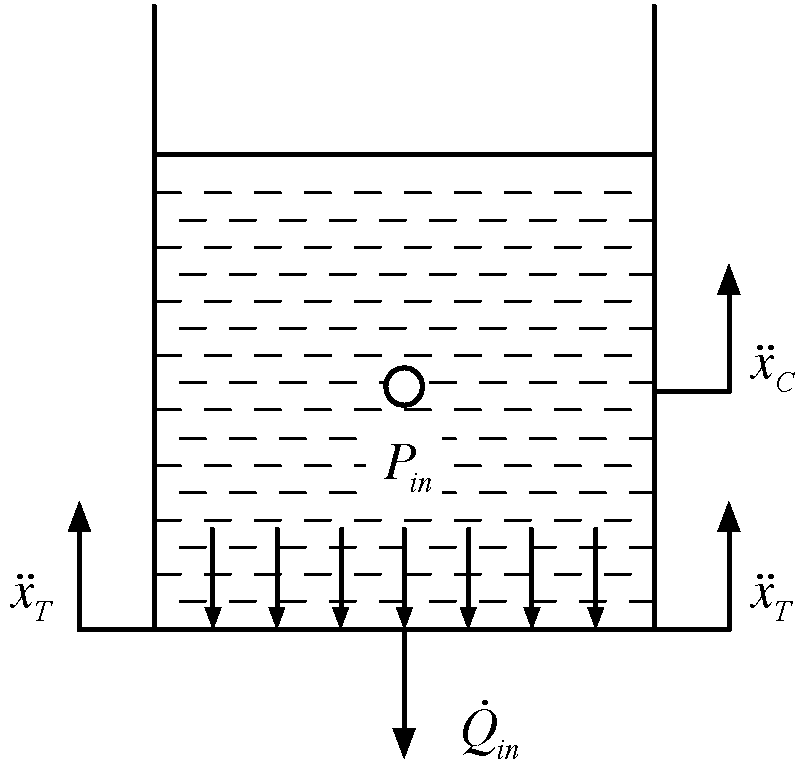
\includegraphics[width=.45\linewidth]{Simplified-Tank-Model.pdf}
  \caption{液体火箭推进剂贮箱简化模型}\label{Simplified-Tank-Model}
\end{figure}

考虑具有刚性平底,部分冲液圆柱形贮箱的轴对称自由振动(如图\ref{Simplified-Tank-Model})。在集中参数模型的描述下,仿照公式\eqref{eq:Inlet-Boundary-Condition},可以写出箱底脉动压力、脉动流量与箱底振动加速度之间的关系:
\begin{equation}
	\label{eq:Tank-Bottom-Relation}
	P_{in}=\rho h_T\left[ \left( 1-\frac{A_{in}}{A_T} \right) \ddot{x}_T- \frac{\dot{Q}_{in} }{A_T} \right]
\end{equation}
公式\eqref{eq:Tank-Bottom-Relation}的推导过程主要基于了以下几点假设:
\begin{itemize}
\item 贮箱为平底,且箱体具有刚性壁面
\item 箱内液体无粘、无旋且不可压缩
\item 同横截面的液体具有相同的运动状态
\end{itemize}
当箱底运动加速度为$\ddot{x}_T$,箱底出口脉动流量变化率为$\dot{Q}_{in}$的时候,贮箱内液体重心加速度满足:
\begin{equation}
	\ddot{x}_C=\frac{(A_T-A_{in})\ddot{x}_T-\dot{Q}_{in} }{A_T}
\end{equation}
根据动量守恒原理,作用在贮箱内液体上的合力应为$\rho h_T A_T\ddot{x}_C $。于是,如果认为贮箱箱底压力为均匀分布,可以很简单的推导出公式\eqref{eq:Tank-Bottom-Relation}的结果:
\begin{equation}
	P_{in}=\frac{(\rho h_T A_T)\ddot{x}_C}{A_T} =\rho h_T\left[ \left( 1-\frac{A_{in}}{A_T} \right) \ddot{x}_T- \frac{\dot{Q}_{in} }{A_T} \right]
\end{equation}
很明显,由于POGO振动问题从本质上看是一种流体与固体之间的强相互作用,所以在该问题的分析过程中必须要考虑贮箱壳体在流体外力作用下的变形情况。此外,由于液体火箭推进剂贮箱底部一般为椭球形,这就使得上述理想情况下的脉动压力--流量关系更加需要修正。

\subsection{带液贮箱的三维建模}
\label{sec:Three-Dimensional-Tank-Model}
同传统的集中参数贮箱模型一样,推进剂贮箱的三维模型同样包括了两个部分:贮箱内部液体与贮箱结构本身。对于前者,为了方便将其综合到耦合系统动力学方程中,此处采用了附加质量法对其进行等效\cite{Brennen:1982, Conca:1997, Liu-Huanzhong:2005}。而对于贮箱结构而言,本节着重介绍了三维模型如何针对贮箱底部开口处进行精细化建模。

\subsubsection{贮箱内部液体建模}
在流体力学中,附加质量法或虚质量法是一种为了简化流固耦合问题的计算而发明的解耦方法。在不考虑液体粘性和可压缩性的条件下,这种方法的特点在于能够生成一种与结构系统湿面单元自由度完全耦合的液体质量矩阵,通过将液体质量矩阵附加到结构系统来达到模拟液体与结构系统相互作用的目的。
\begin{figure}[!tb]
  \centering
  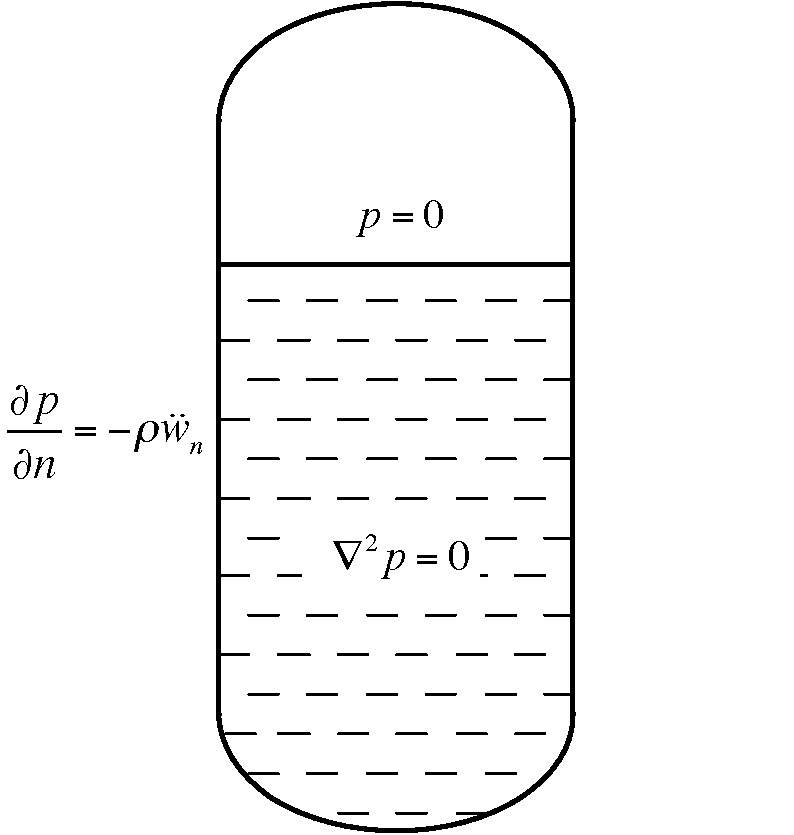
\includegraphics[width=.5\linewidth]{General-Liquid-Tank.pdf}
  \caption{带液贮箱压力分布示意图}\label{General-Liquid-Tank}
\end{figure}

假设贮箱内的液体无粘、无旋且不可压缩,不考虑液体自由面晃动,箱体内(如图\ref{General-Liquid-Tank})流体压力场$p(x,y,z)$应该满足:
\begin{equation}
	\label{eq:Liquid-Laplace-Equation}
	\begin{cases}
	\nabla^2p=0 & \text{液体内部}\\
	{\displaystyle \frac{\partial p}{\partial n}}=-\rho \ddot{w}_n & \text{箱体接触面} \\
	p=0 & \text{液体自由面}
	\end{cases}
\end{equation}

为了求解控制流体压力场分布的Laplace方程,可以利用源、汇和偶极子的奇点配置法\cite{Morand:1995, Ohayon:1995, Ohayon:2004},首先将一系列的源分布到结构系统湿面的表面节点上,其中每个源所产生的解均满足拉普拉斯方程。然后,通过求解关于源强度的线性方程组,使得这一系列源在固液边界处所产生的流体运动速度满足前面提到的势函数边界条件。

假设位于$\boldsymbol{r}_j$位置的源强度为$\sigma_j$,那么在该源影响下任意位置$\boldsymbol{r}_i$处的流体速度$\dot{\boldsymbol{u}}_i$可以表达为:
\begin{equation}
	\label{eq:Laplace-Velocity-Holmholtz}
	\dot{\boldsymbol{u}}_i=\sum_j \int_{A_j} \frac{\sigma_j\boldsymbol{e}_{ij}}{{\| \boldsymbol{r}_i-\boldsymbol{r}_j \|}^2}\ud A_j
\end{equation}
其中$\boldsymbol{e_{ij}}$是从位置$\boldsymbol{r}_j$到$\boldsymbol{r}_i$的单位向量,源$\sigma_j$的作用范围为$A_j$。

由于贮箱内部液体压力由Laplace方程\eqref{eq:Liquid-Laplace-Equation}所决定,考虑到流体在靠近壁面处的速度连续性边界条件,非定常压力场$p(x,y,z,t)$可由结构系统的运动状态唯一确定。借助公式\eqref{eq:Laplace-Velocity-Holmholtz},流体压力场从形式上可以表示为:
\begin{equation}
	p(x,y,z,t)=-{\boldsymbol{P}}(x,y,z)\ddot{\boldsymbol{x}}_s(t)
\end{equation}
其中$\ddot{\boldsymbol{x}}_s(t)$是与液体相关联的箱体节点加速度。引入合适的形函数$\boldsymbol{N}^{\ut}(x,y,z)$,可以获得液体作用于贮箱壁面的等效节点力:
\begin{equation}
	\boldsymbol{f}_L(t)=\int_\Gamma -\boldsymbol{N}^{\ut}(x,y,z) \boldsymbol{P}(x,y,z)\ddot{\boldsymbol{x}}_s(t)\ud \Gamma
\end{equation}
经过单元组装,可以获得液体的附加质量矩阵:
\begin{equation}
	\label{eq:Equivalent-Added-Mass}
	\boldsymbol{F}_L(t)=-\boldsymbol{M}_a \ddot{\boldsymbol{x}}_s(t)
\end{equation}
可以看出,方程\eqref{eq:Equivalent-Added-Mass}具有与常规结构系统动力学公式一致的二阶微分方程形式,这将为后续耦合系统的稳定性分析带来巨大便利。

\subsubsection{贮箱壳体的三维建模}
\label{sec:3D-Model-Hulk}
\begin{figure}[!htb]
  \centering
  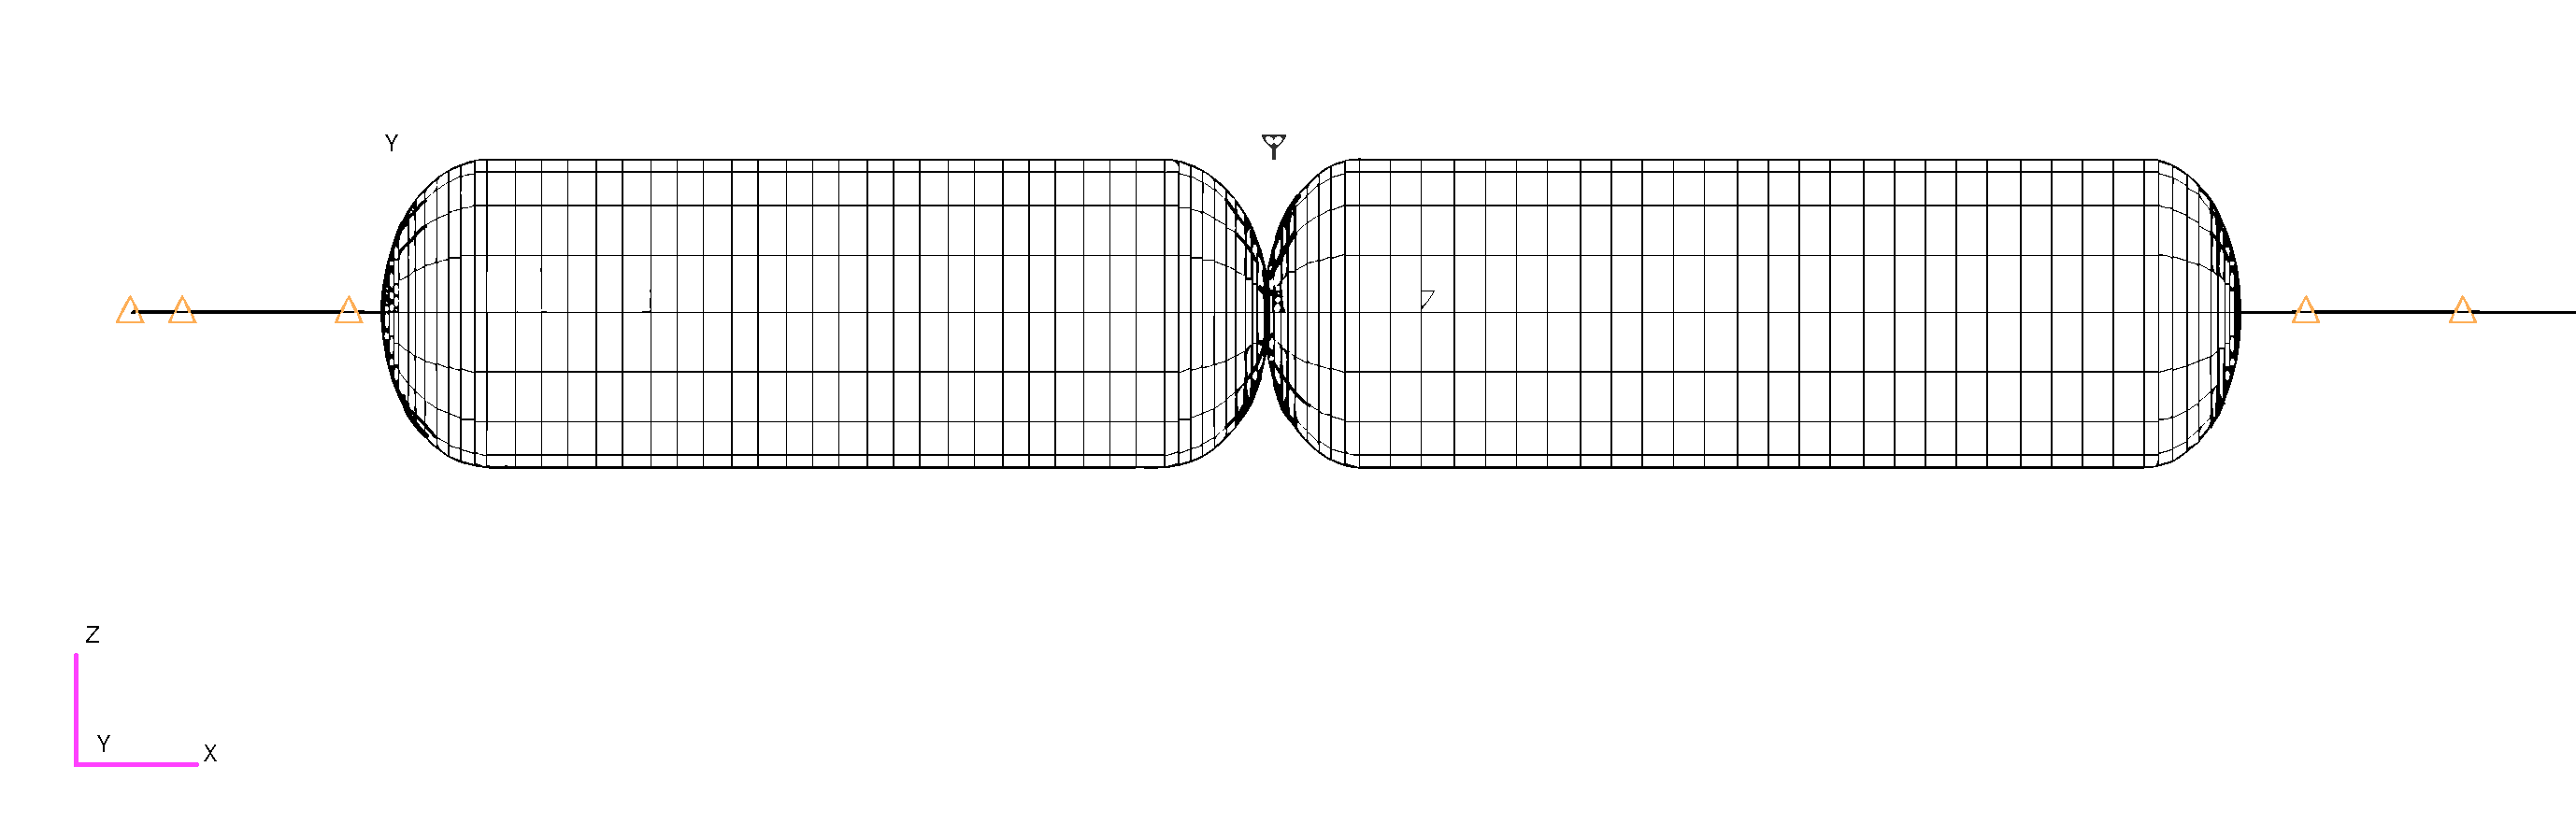
\includegraphics[width=\linewidth]{Liquid-Tank-FEM-MSC.pdf}
  \caption{推进剂贮箱三维有限元模型}\label{Liquid-Tank-FEM-MSC}
\end{figure}

贮箱壳体的三维有限元模型如图\ref{Liquid-Tank-FEM-MSC}所示。推进剂贮箱除底部开口处外均采用Shell单元模拟,三维模型在箱体后短壳处用REB2单元\footnote{既将推进剂贮箱与火箭主体部分刚性连接}与集中质量模型相连接。为了方便后续分析充分利用贮箱的轴对称特性,在氧化剂与燃烧剂贮箱箱底分别建立柱坐标系,并指定其做为各自壳体Shell单元的局部分析坐标系。

\begin{figure}[!htb]
  \centering
  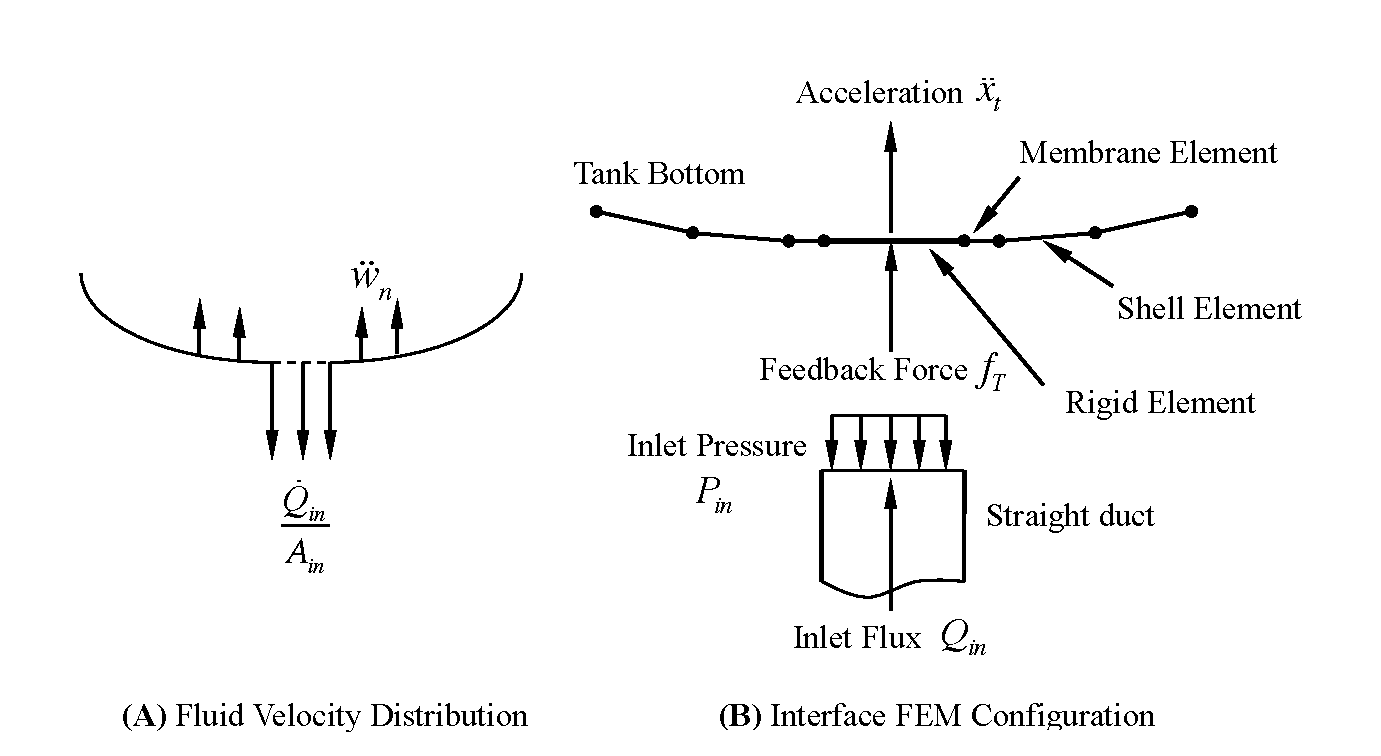
\includegraphics[width=\linewidth]{FEM-Tank-Bottom.pdf}
  \caption{推进剂箱底的精细化建模}\label{FEM-Tank-Bottom}
\end{figure}

\begin{figure}[!htb]
  \centering
  \setlength{\fboxrule}{0.8pt}
  \fbox{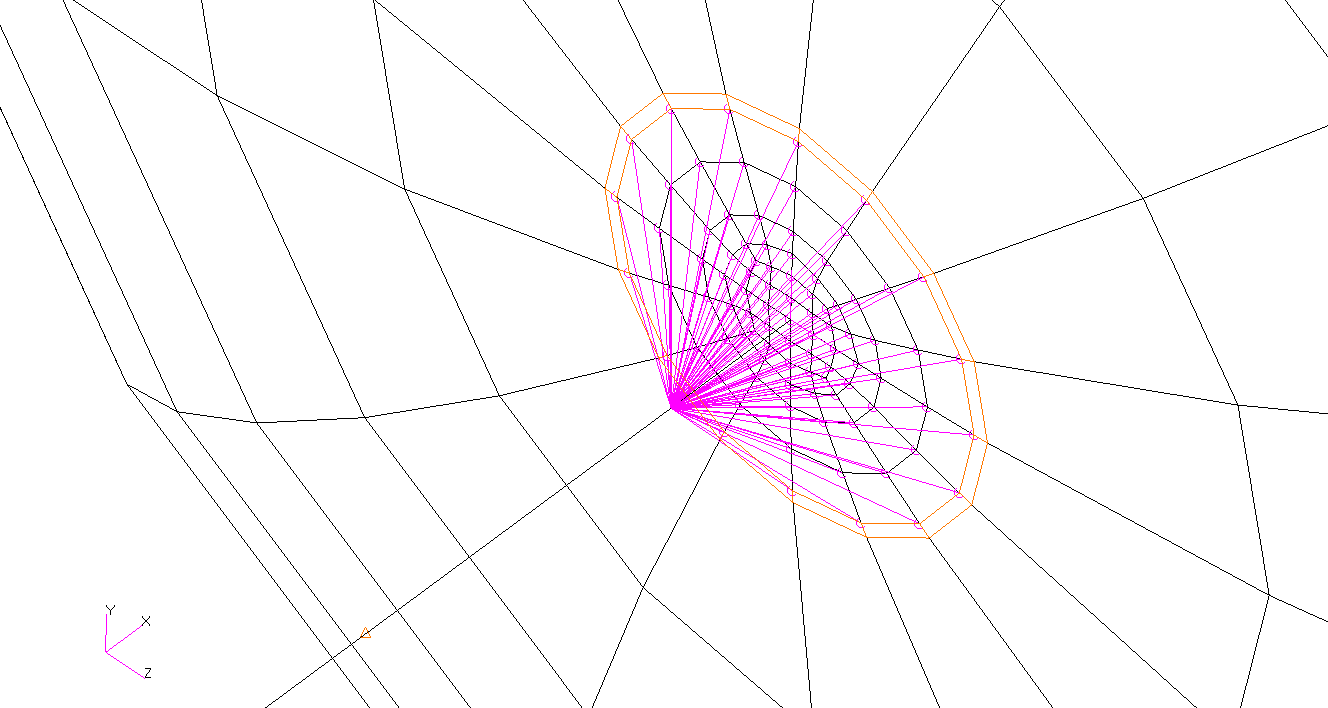
\includegraphics[width=.8\linewidth]{Patran-Tank-Bottom.png}}
  \caption{贮箱底部开口处的有限元模型}\label{Patran-Tank-Bottom}
\end{figure}

由以上分析可以得知,刚性单元的法向加速度$\ddot{x}_T$与管路系统入口端流量变化率$\dot{Q}_{in}$\footnote{这里需要注意相对流量和绝对流量的概念:相对流量是指通过某个随体截面的液体流量,而绝对流量指的是通过某个固定截面的液体流量。在管路系统传递方程的推导过程中,$Q^{(n)}$都被用作指代绝对流量,此处$Q_{in}$也是如此}之间存在如下关系:
\begin{equation}
	\dot{Q}_{in}\footnote{从表面上看,公式中$Q_{in}$应该代表的是相对于刚体活塞截面的管路入口端相对流量,不过由于在推进剂贮箱和管路系统主管的连接处通常加装有波纹管等缓冲设备(图\ref{POGO-PipeLine}未反映),因而刚体单元的截面恰好可以认为是相对管路系统静止的,从而$Q_{in}$可以作为主管的入口端绝对流量}
	=A_{in}\ddot{x}_T 
\end{equation}
进而可以得出脉动压力对结构系统的反馈力可以简单的表示为:
\begin{equation}
	\label{eq:3D-Pressure-Feedback-Force}
	F_p=A_{in}P_{in}
\end{equation}

\begin{figure}[!htb]
  \centering
  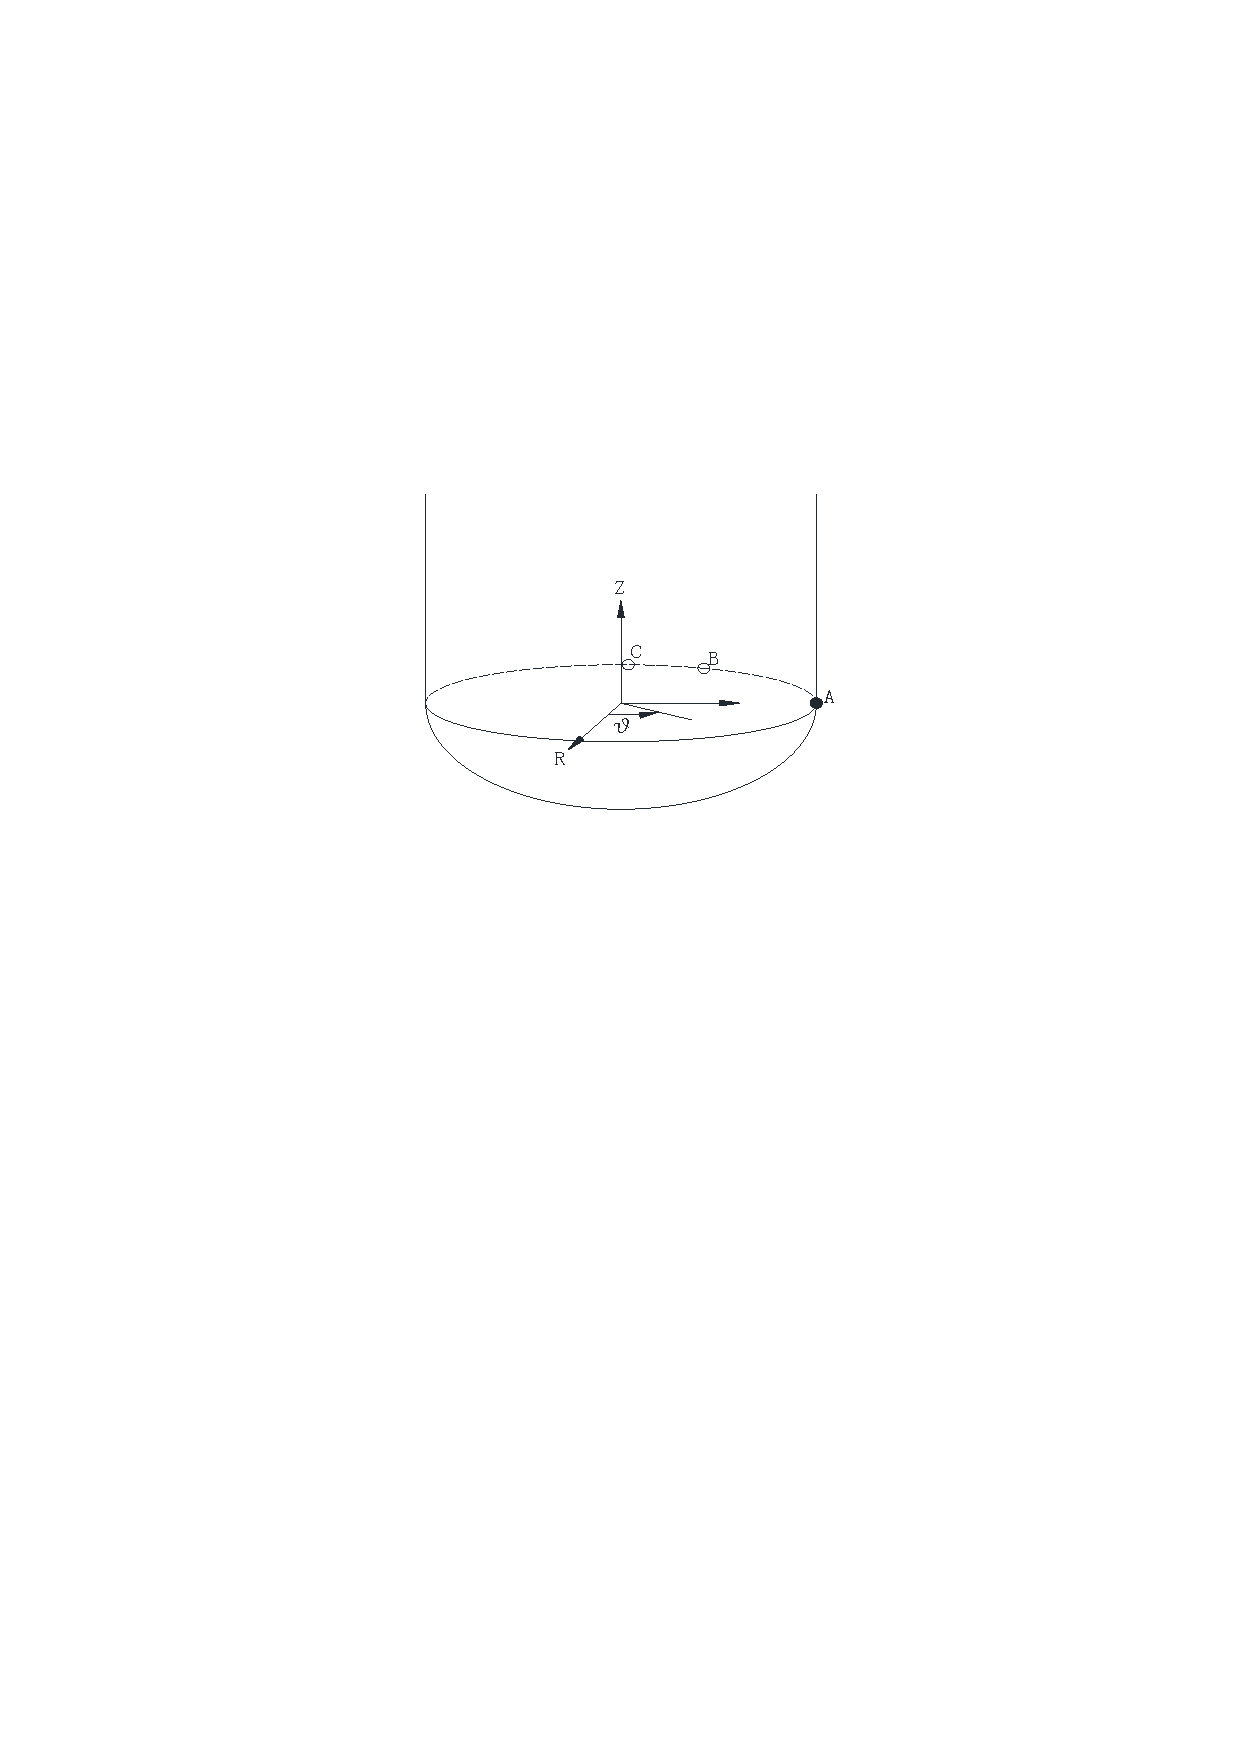
\includegraphics[width=.4\linewidth]{Axial-Symmetric-Tank-Model.pdf}
  \caption{柱坐标系下的轴对称贮箱示意图}\label{Axial-Symmetric-Tank-Model}
\end{figure}

由于POGO稳定性分析主要关心的是液体火箭耦合系统的纵向振动,所以对于结构系统模型中除去三维贮箱的其他集中参数节点,仅允许其产生纵向运动而约束了其余自由度。对于贮箱模型中的壳体单元,因为实际液体火箭贮箱本身通常具有良好的轴对称性,所以此处对其做出了如下简化处理(如图\ref{Axial-Symmetric-Tank-Model}):以贮箱轴线为$z$轴建立柱坐标系,贮箱上的节点位移均参考此坐标系;在贮箱模型的周向一圈节点中,选择一个独立点A,其余节点B,C等均通过MPC约束其轴向位移到A点。此外,为了防止贮箱产生不必要的扭转运动,模型还约束住了贮箱壳体单元沿轴线方向的扭转自由度。可以预见的是,这样的处理手段既能够缩减掉推进剂贮箱大量的无用自由度,又能够保证贮箱产生合理的纵向运动和横向轴对称运动,基本做到了效率显著提升而又兼顾结果精确性。此外,由于该有限元模型的分析结果自动过滤了与POGO无关的贮箱局部模态,所以可以很方便的将其与传统方法得到的稳定性分析结果进行对比,利于后续分析。

\subsection{三维贮箱模型的方法验证}
为了验证节\ref{sec:Three-Dimensional-Tank-Model}建立三维贮箱模型的正确性,并指出其将为耦合系统的稳定性分析带来哪些改进,本节拟从以下两点进行论述:
\begin{itemize}
\item 验证三维贮箱模型的固有频率及模态是否合理
\item 指出该模型为管路系统反馈力计算带来的改进
\end{itemize}

\begin{table}[htbp]
	\renewcommand{\arraystretch}{1.3}
	\caption{液体火箭结构系统固有频率的计算结果对比}
	\centering
	\begin{minipage}[t]{\linewidth}
	\begin{tabular}{cccc:cc}
		\toprule
		\multicolumn{4}{c}{三维贮箱模型} & \multicolumn{2}{c}{集中参数模型} \\
		\cmidrule(r{0.5em}){1-4}  \cmidrule(l{0.5em}){5-6} 
		MODE NO. & CYCLES & MODE NO. & CYCLES & MODE NO. & CYCLES \\
		\midrule
		1     & \framebox{\textcolor{red}{0}}     & 11    & 29.6  & 1     & \textcolor{red}{0}    \\
		2     & 2.58  & 12    & 30.3  & 2     & \textcolor{red}{9.08} \\
		3     & \framebox{\textcolor{red}{8.49}}  & 13    & \framebox{\textcolor{red}{36.1}}  & 3     & \textcolor{red}{11.2} \\
		4     & \framebox{\textcolor{red}{9.32}}  & 14    & 36.6  & 4     & \textcolor{red}{20.1} \\
		5     & 16.3  & 15    & 36.8  & 5     & \textcolor{red}{34.8} \\
		6     & 16.6  & 16    & 37.6  & 6     & \textcolor{red}{39.7} \\
		7     & 17.8  & 17    & \framebox{\textcolor{red}{39.3}}  & 7     & \textcolor{red}{65.4} \\
		8     & \framebox{\textcolor{red}{20.2}}  & 18    & 40.2  & 8     & \textcolor{red}{72.5} \\
		9     & 23.1  & 19    & 41.4  & 9     & \textcolor{red}{93.9} \\
		10    & 29.2  & 20    & 44.6  & 10    & \textcolor{red}{110} \\
		\bottomrule
	\end{tabular}
	\end{minipage}

	\vspace{2em}

	\centering
	\begin{minipage}[t]{\linewidth}
	\begin{tabular}{cccccc}
		\toprule
		\multicolumn{6}{c}{三维贮箱模型} \\
		\cmidrule{1-6}
		MODE NO. & CYCLES & MODE NO. & CYCLES & MODE NO. & CYCLES \\
		\midrule
		21    & 48    & 31    & \framebox{\textcolor{red}{63.8}}  & 41    & 87 \\
		22    & 49.6  & 32    & 67.4  & 42    & 89.5 \\
		23    & 49.7  & 33    & 68.9  & 43    & \framebox{\textcolor{red}{91.2}} \\
		24    & 51.1  & 34    & 71.4  & 44    & 95.8 \\
		25    & 53.6  & 35    & \framebox{\textcolor{red}{73.1}}  & 45    & 96.9 \\
		26    & 55    & 36    & 74.8  & 46    & 99.8 \\
		27    & 55.4  & 37    & 77.2  & 47    & 103.3 \\
		28    & 57.1  & 38    & 82.5  & 48    & 103.7 \\
		29    & 60.2  & 39    & 82.9  & 49    & 105.9 \\
		30    & 62.8  & 40    & 82.9  & 50    & \framebox{\textcolor{red}{108.2}} \\
		\bottomrule
	\end{tabular}
	\end{minipage}
	\label{table:Liquid-Rocket-Structural-System-Eigen}
\end{table}

\section{三维贮箱对应的管路系统模型}
\label{sec:3D-Tank-VS-Feedline-Update}

\begin{figwindow}[0,r,{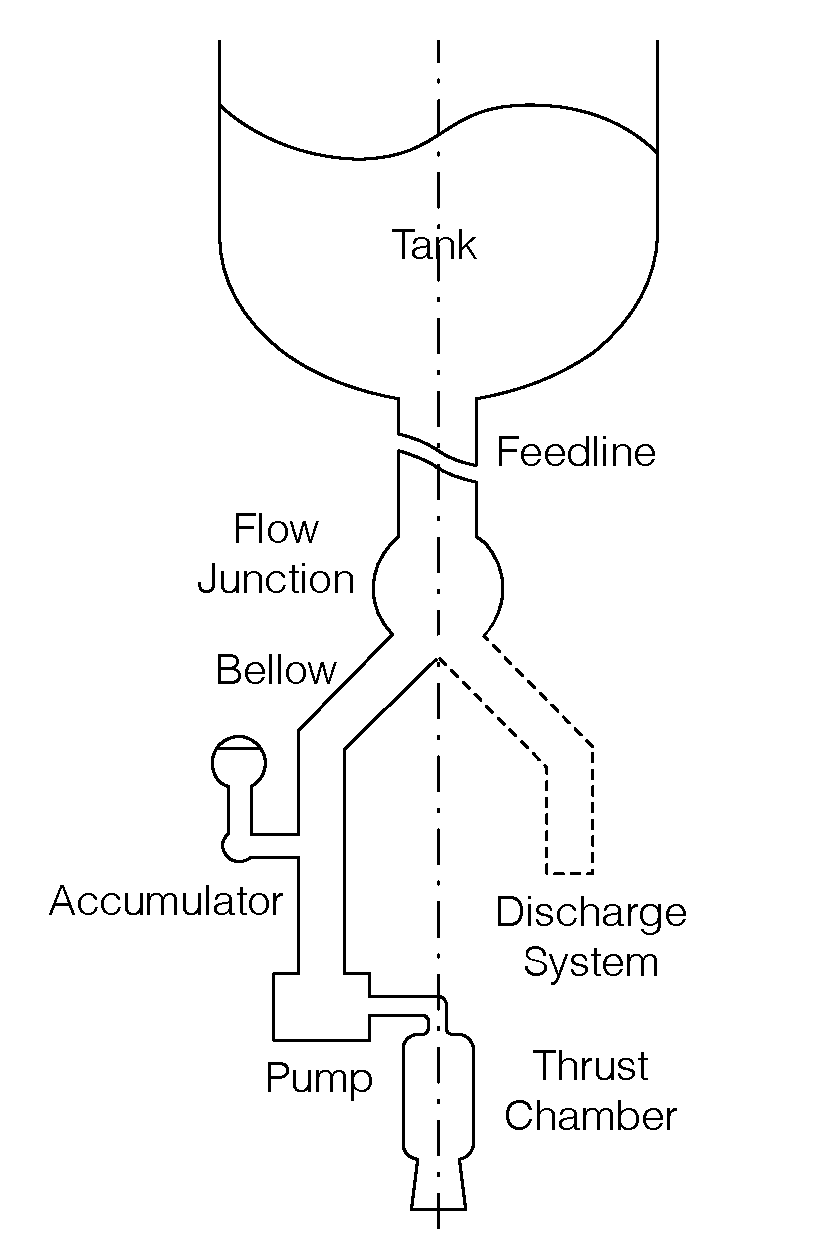
\includegraphics[width=.5\linewidth]{3D-Feedlink-Scheme}},{管路推进系统结构示意图\label{3D-Feedlink-Scheme}}]
类似节\ref{sec:Lumped-Feedline-Model},与三维推进剂贮箱对接的管路系统如图\ref{3D-Feedlink-Scheme}所示。本节沿用了之前管路元件传递函数的处理手段,首先采用有理分式拟合方法对三维贮箱对应的管路系统在形式上进行初步整理。由于液体贮箱的分析平台基于有限元分析软件MSC.Nastran,观察到其动态建模方法中提供了TF卡技术来直接修改系统整体矩阵,所以此处并没有继续采用类结构化方法处理有理分式形式的管路系统反馈力,而是利用构造TF卡的手段将其耦合到液体火箭结构系统之中。

\makebox[2\Han]{}不同于公式\eqref{eq:Feedback-Force-Transfer},由于三维贮箱不需要考虑箱底脉动流量引起反馈力,管路系统反馈力形式变为:
\protect\phantom{占座 占座 占座 占座 占座 占座 占座 占座 }

\end{figwindow}

\begin{equation}
	\label{eq:3D-Feedback-Force-Transfer}
	\boldsymbol{F}_p(s)=\left[ \begin{matrix}
	   F_2(s)  \\
	   F_3(s)  \\
	   F_4(s)  \\
	\end{matrix} \right]  \triangleq \boldsymbol{R}_{pq}(s)\left[ \begin{matrix}
	   \dot{x}_T(s)  \\
	   \dot{x}_{L1}^{(5)}(s)  \\
	\end{matrix} \right] \triangleq \boldsymbol{R}_{pq}(s)\boldsymbol{\dot{X}}_q(s)
\end{equation}

利用所得反馈力传递关系的有理分式形式,可以将公式\eqref{eq:3D-Feedback-Force-Transfer}与结构系统进行耦合:
\begin{equation}
	\left \{
	\label{eq:3D-Coupled-System-Transfer}
	\begin{aligned}
	\left[s^2 \boldsymbol{M}_s+ s\left(\boldsymbol{C}_s+\boldsymbol{\dot{M}}_s
	-\boldsymbol{L}_{sp} \boldsymbol{R}_{pq}(s)\boldsymbol{L}_{qs}\right)+ \boldsymbol{K}_s \right]\boldsymbol{X}_s(s)&=\boldsymbol{F}_s(s) \\
	s\boldsymbol{M}_{pq}+ \boldsymbol{D}_{pq}+ \sum_{k=1}^n
	\left( \frac{\boldsymbol{C}_{pq}^{(k)}}{s-\boldsymbol{A}_k} +
	\frac{\bar{\boldsymbol{C}}_{pq}^{(k)}}{s-\bar{\boldsymbol{A}}_k}  \right)
	+ \sum_{j=1}^{m}\frac{\boldsymbol{B}_{pq}^{(j)}}{s-R_j}&=\boldsymbol{R}_{pq}(s)
	\end{aligned} \right.
\end{equation}

相比集中参数管路模型,这里采用的有理分式更具通用性,考虑了传递关系中可能包含实数零点的一般情况。接下来,对于此处所得有理分式,将引入MSC.Nastran中的TF卡建模方法来对其进行进一步处理。

考察公式\eqref{eq:3D-Coupled-System-Transfer}中传递矩阵$\boldsymbol{R}_{pq}$的任一元素$R_{pq}$
\begin{equation}
	R_{pq}=T(s)=\left( sM_0 + D_0 + \sum_{k=1}^n \frac{C_k}{s-A_k}+ \sum_{k=1}^{n}\frac{\bar{C}_k}{s-\bar{A}_k} + \sum_{j=1}^{m} \frac{B_j}{s-R_j} \right) 
\end{equation}
分离实、虚部,可以使得$T(s)$中不再含有TF方法所不能处理的复数系数\footnote{由于TF卡建模方法仅支持位移传递函数的输入,而传递矩阵$\boldsymbol{R}_{pq}$表示的是速度反馈,所以在$T(s)$中分子分母同时乘以$s$以便后续处理}
\begin{equation}
	\label{eq:3D-Transfer-Single-Rational}
	T(s)=\frac{1}{s} \left[ (sM_0+D_0)s+ \sum_{k=1}^{n} \frac{2(C'_ks^2-C'_kA'_k s-C''_kA''_k s)}{s^2-2A'_ks+{A'_k}^{2}+{A''_k}^2}+\sum_{j=1}^m \frac{B_js}{s-R_j} \right]
\end{equation}
鉴于Nastran中传递函数的标准写法为($u$为节点位移):
\begin{equation}
	\label{eq:Standard-Nastran-TF}
	(B_0+B_1s+B_2s^2)u_d+\sum_i (A_{0i}+A_{1i}s+ A_{2i}s^2)u_i=0
\end{equation}
借助Epoint(辅助点)$x_1^0(t),x_{2}^k(t),x_{3}^j(t)$,其中
\begin{equation}
	\label{eq:Epoint-Relationship}
	\begin{aligned}
		X_1^0(s)&=\Laplace{x_1^0(t)}= (s^2M_0+D_0s)X_q(s) \\
		X_{2}^k(s)&=\Laplace{x_2^k(t)}= X_q(s)/(s^2-2A'_ks+{A'_k}^2+{A''_k}^2)\\
		X_{3}^j(s)&=\Laplace{x_3^j(t)}= X_q(s)/(s-R_j)
	\end{aligned}
\end{equation}
可以利用公式\eqref{eq:3D-Transfer-Single-Rational}写出传递矩阵$T(s)$对于反馈力$\boldsymbol{F}_p(s)$的贡献:
\begin{equation}
	\label{eq:Quasi-Structural-Epoint}
	\begin{aligned}
		f^{q}(s)&= T(s)\dot{X}_q(s) =X_1^0(s) + \sum_{j=1}^m (B_js)X_3^{j}(s) \\
		&+\sum_{k=1}^n 2(C'_k s^2- C'_k A'_k s- C''_k A''_ks)X_2^{k}(s)
	\end{aligned}
\end{equation}
考虑到传递矩阵$\boldsymbol{R}_{pq}$中各个分量的极点是相同的,为了尽可能少的引入Epoint,在对其整体进行TF卡片输入的时候,辅助点$\tilde{\boldsymbol{X}}(s)$的引入规范如下:
\begin{equation}
	\label{eq:General-Epoint-Relationship}
	\begin{aligned}
		{\tilde{X}}_{pq}^{(0)}(s)&=(s^2M_{pq}+D_{pq}s)X_q(s) \\
		{\tilde{X}}_{q}^{(k)}(s)&=X_q(s)/(s^2-2A'_ks+{A'_k}^2+{A''_k}^2)\\
		{\tilde{X}}_{q}^{(j)}(s)&=X_q(s)/(s-R_j)
	\end{aligned}
\end{equation}
可知辅助点的总数目为$p\cdot q+ q\cdot k+ q\cdot j$。TF卡片的示例样式如图\ref{TF-Card-Construction}。

\begin{figure}[!htb]
  \centering
  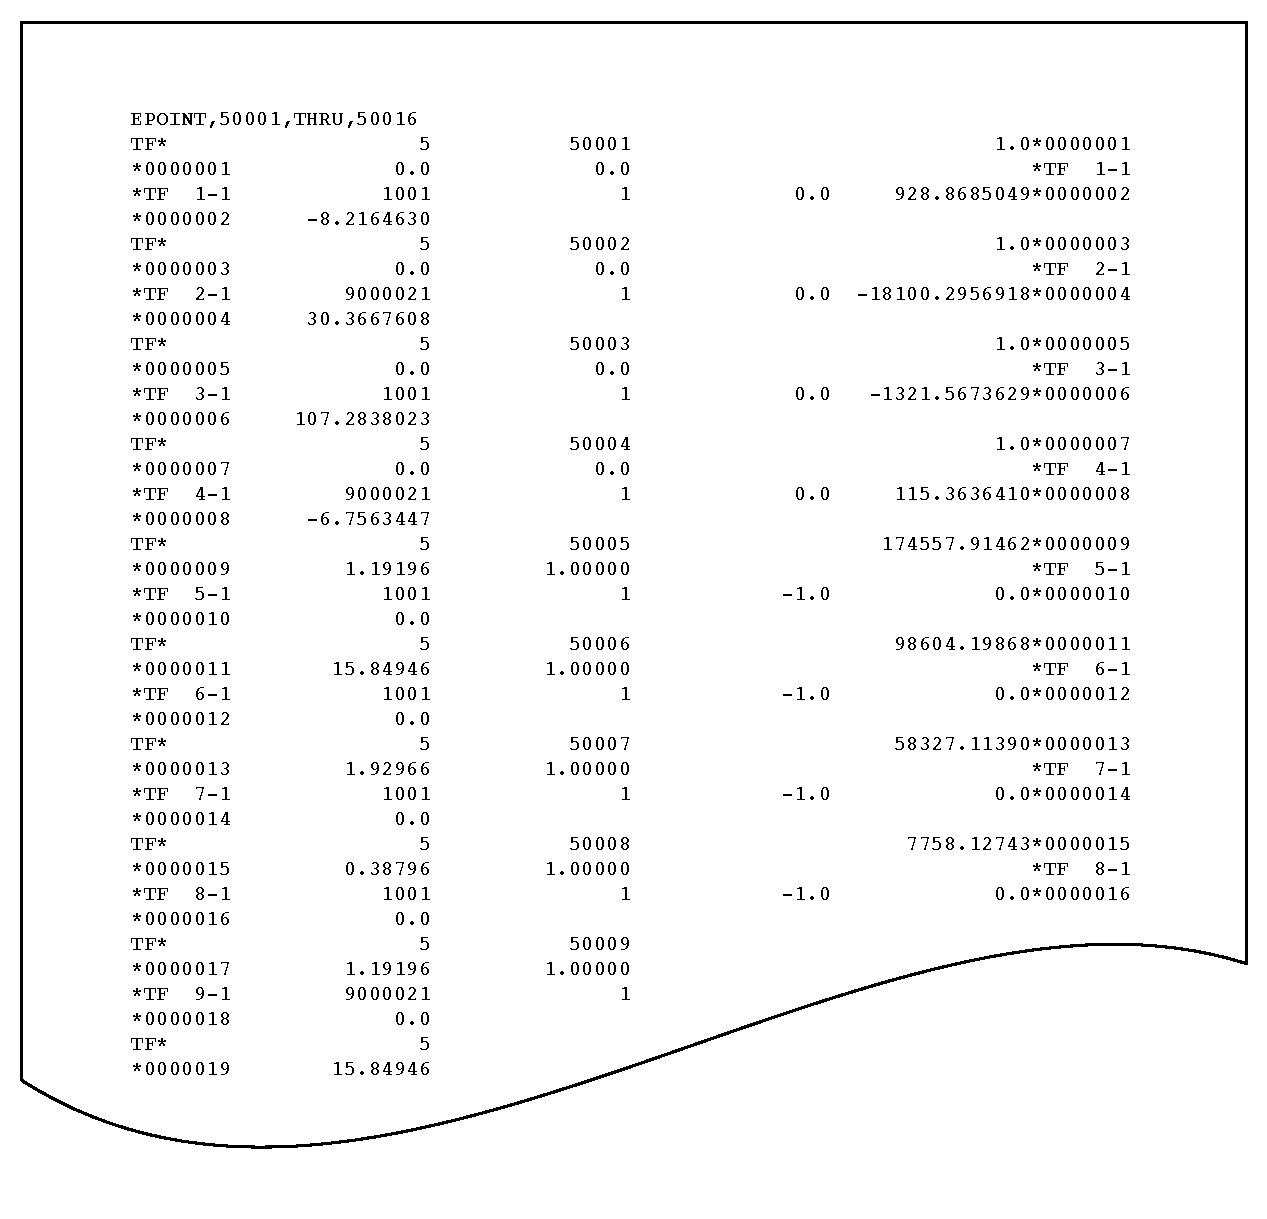
\includegraphics[width=\linewidth]{TF-Card-Construction}
  \caption{MSC.Nastran传递函数TF卡片构造示例}\label{TF-Card-Construction}
\end{figure}

最后,可利用公式\eqref{eq:General-Epoint-Relationship},写出传递矩阵$\boldsymbol{R}_{pq}$中任意元素$R_{pq}$对于反馈力$\boldsymbol{F}_p(s)$的贡献:
\begin{equation}
	\label{eq:General-Quasi-Structural-Epoint}
	\begin{aligned}
		f_{pq}(s)&= R_{pq}\dot{X}_q(s)={\tilde{X}}_{pq}^{(0)}(s) + 
		\sum_{j=1}^m (B_{pq}^{(j)}s){\tilde{X}}_{q}^{(j)}(s) \\
		&+\sum_{k=1}^n 2(C_{pq}^{\prime (k)} s^2- C_{pq}^{\prime (k)} A'_k s- C_{pq}^{\prime\prime(k)} A''_ks){\tilde{X}}_{q}^{(k)}(s)
	\end{aligned}
\end{equation}
观察公式\eqref{eq:General-Epoint-Relationship}和\eqref{eq:General-Quasi-Structural-Epoint},可见其均满足Nastran的输入要求\eqref{eq:Standard-Nastran-TF}。于是,方程\eqref{eq:3D-Coupled-System-Transfer}最终可以被划归为二阶常微分方程组的传递矩阵形式:
\begin{equation}
	\label{eq:3D-Final-Coupled-Transfer-Function}
	(s^2\boldsymbol{M}_c+s\boldsymbol{C}_c+\boldsymbol{K}_c)\boldsymbol{X}_c(s)=\boldsymbol{F}_c(s)
\end{equation}
其中,$\boldsymbol{X}_c(s)=\left[ \boldsymbol{X}_s^{\ut}(s)\quad \tilde{\boldsymbol{X}}^\ut(s) \right]^{\ut}$为包含辅助点自由度的增广节点位移向量,$\boldsymbol{M}_c,\boldsymbol{C}_c,\boldsymbol{K}_c$为重新装配后的耦合系统质量、阻尼和刚度矩阵。可以看到,由于辅助变量的引进,耦合系统整体矩阵不再保持原有的对称性,所以通常需要利用成熟的复模态求解方法对其进行复特征值和特征向量的求解。不过,相对于求解管路系统原始的非线性反馈力传递矩阵而言,Nastran等商业有限元软件的计算效率和求解精度都要远远胜出。

\section{耦合系统阻尼特性分析}
随着充液航天器的发展,带液贮箱的阻尼特性分析正引起越来越多研究者的关注。然而,由于人们对于物质在其运动过程中能量耗散的成因及机理分析还很不完善,以至于就单纯的结构或者流体动力学问题而言,系统阻尼的建模、校核与评估通常即为求解问题中最难处理的一部分。对于POGO振动问题,由于液体火箭的结构阻尼一般是由实验测定得出,所以此处本节着重介绍了贮箱内部液体的阻尼计算。

\subsection{液体阻尼特性分析基础}
在节\ref{sec:Three-Dimensional-Tank-Model}介绍的带液贮箱建模过程中,由于本文的研究重点为液体火箭的纵向耦合振动,所以模型并没有考虑贮箱内部液体晃动等与耦合系统纵向振动联系较弱的其他运动形式。然而,针对贮箱内部液体的阻尼建模问题,因为液体阻尼主要与箱体壁面粘性阻尼作用、自由液面处的粘性耗散、液体内部粘性耗散及毛细作用等四个方面相关联\cite{Henderson:1994, Martel:1998},所以此时必须将贮箱内液体的晃动等方面考虑进来。

该方法认为理想流体区域的运动由Laplace方程控制($\Phi$为速度势):
\begin{equation}
	\label{eq:Ideal-Liquid-Laplace}
	\left \{
	\begin{alignedat}{2}
	&\nabla^2\Phi=0 &\quad &\text{液体内部}\:\Omega\\
	&{\displaystyle \frac{\partial \Phi}{\partial n}}=0 &\quad &\text{不可渗透边界条件}\:S_w \\
	&{\displaystyle \frac{\partial \Phi}{\partial t}}=-gh  &\quad &\text{液体自由面}\:S_f
	\end{alignedat} \right.
\end{equation}
对于Stokes边界层,由于其厚度在一般情况下非常薄,因此可以将壁面边界层内某一点的流动速度近似处理为于壁面平行:
\begin{equation}
	\frac{\partial \boldsymbol{v}}{\partial t} = \nu\frac{\partial^2 \boldsymbol{v}}{\partial z^2}
\end{equation}
其中$\boldsymbol{v}$为流体速度,$z$为壁面法向坐标,$\nu$为液体的运动学粘度系数。根据计算所得的流体运动情况,就可以计算Stokes边界层与流体内部粘性的能量耗散。

\begin{enumerate}[label=\textbf{\Roman*.}, align=left, leftmargin=0pt, listparindent=\parindent, itemindent=!, labelwidth=\parindent, labelsep=0pt, itemsep=1em]
\litem{Stokes边界层能量耗散}
\begin{itemize}
\item 对于液面没有受到污染的情况:仅在壁面上计算Stokes边界层。若假设$\boldsymbol{v}=\boldsymbol{U}e^{i\omega t}$,一个晃动周期内的平均能量耗散率为
\begin{equation}
	D_1=\rho\sqrt{\frac{1}{8}\nu\omega}\iint_{S_w}| \boldsymbol{U}|^2\ud S
\end{equation}
\item 对于自由液面受到污染的情况:需要额外考虑自由液面处的Stokes边界层能量耗散
\begin{equation}
	D_1=\rho\sqrt{\frac{1}{8}\nu\omega}\iint_{S_w+S_f}| \boldsymbol{U}|^2\ud S
\end{equation}
\end{itemize}

\litem{流体内部的能量耗散}
\begin{itemize}
\item[]对于流体的粘性耗散有如下耗散函数:
\begin{equation}
	F=\frac{\mu}{2}\int_{\Omega}\mathfrak{R}(\boldsymbol{v})\ud\Omega
\end{equation}
其中$\mu$为动力学粘度系数,$\boldsymbol{v}=\left[ \begin{matrix} v_x & v_y & v_z \end{matrix} \right]^\ut$
\begin{displaymath}
	\begin{aligned}
		\mathfrak{R}(\boldsymbol{v})=&2\left[(\frac{\partial v_x}{\partial x})^2 + (\frac{\partial v_y}{\partial y})^2+ (\frac{\partial v_z}{\partial z})^2\right] \\
		&+ (\frac{\partial v_z}{\partial y}- \frac{\partial v_y}{\partial z})^2+(\frac{\partial v_x}{\partial z}- \frac{\partial v_z}{\partial x})^2 + (\frac{\partial v_y}{\partial x}- \frac{\partial v_x}{\partial y})^2
	\end{aligned}
\end{displaymath}
利用方程\eqref{eq:Ideal-Liquid-Laplace},可以写出一个周期内液体内部的平均能量耗散率为:
\begin{equation}
	\begin{aligned}
		D_2&=\frac{\omega}{2\pi}\int_0^{\frac{2\pi}{\omega}}2F(\Phi)\ud t \\
		&=\frac{\omega}{2\pi}\int_0^{\frac{2\pi}{\omega}}\mu\int_\Omega \mathfrak{R}(\Phi)\ud \Omega \cos ^2 (\omega t)\ud t \\
		&=\frac{1}{2}\mu\int_\Omega\mathfrak{R}(\Phi)\ud \Omega
	\end{aligned}
\end{equation}
\end{itemize}
\end{enumerate}
如此,由于在一个周期内液体晃动的总机械能为
\begin{equation}
	E=\frac{\rho}{2}\int_\Omega |\nabla \Phi|^2\ud \Omega
\end{equation}
可以计算出贮箱内液体阻尼比$\gamma$为\cite{Abramson:1966, Miles:1958}:
\begin{equation}
	\label{eq:Damping-Ratio-Stokes}
	\gamma=\frac{D_1+D_2}{2\omega E}
\end{equation}
实际上,Abramson早在1966年便通过实验数据的拟合,给出了圆柱容器内液体小幅晃动第一阶模态阻尼的经验公式\cite{Abramson:1966}:
\begin{equation}
	\label{eq:Empirical-Damping-Ratio}
	\delta=4.98\nu^{1/2}R^{-3/4}g^{-1/4}\left[ 1+\frac{0.318}{\sinh (1.84{\displaystyle\frac{h}{R}})} \left( \frac{1-{\displaystyle\frac{h}{R}}}{\cosh(1.84{\displaystyle\frac{h}{R}})} +1\right) \right]
\end{equation}
其中$R$为容器的半径,$h$为容器内部液体高度,$g$为当地重力加速度。经过验证,在$\displaystyle \frac{h}{R}<1.0$的时候,公式\eqref{eq:Damping-Ratio-Stokes}与\eqref{eq:Empirical-Damping-Ratio}给出的计算结果相当一致\cite{WangWei:2005,WangWei:2006}。但是,由于上述Henderson模型建立在线性化自由表面边界的基础之上,所以其结论仅局限在液面做小幅晃动的时候。对于$\displaystyle \frac{h}{R}>1.0$的情况,Abramson给出了另外的经验公式:
\begin{equation}
	\delta=4.98\nu^{1/2}R^{-3/4}g^{-1/4}
\end{equation}
由此可见,现阶段可以通过理论推导来获得的阻尼模型还很有限,计算模型的验证还远远离不开实验去验证。

\subsection{带防晃板的贮箱液体阻尼}
Mikishev和Stephens等人经过大量的科学实验,发现液体的粘性耗散作用其实在防止液体晃动方面真正能起到的作用非常有限\cite{Mikishev:1961, Stephens:1962}。在正常规格的贮箱内部,即使内部装有动力学粘度超出水一百倍的液体,其粘性阻尼也不会超过0.5\si{\percent}。因而,对于液体火箭这种需要严格控制液体晃动的复杂构型,Baffle(防晃板)的使用是必不可少的。

存在防晃板的液体建模其实与公式\eqref{eq:Ideal-Liquid-Laplace}非常类似,获得解析解的技术手段一般也即为时间-空间分离变量法。若在贮箱根部建立$rz\theta$柱坐标系,假设贮箱底部存在$\ddot{x}(t)=\ddot{x}_0e^{\num{i}\omega t}$的简谐运动,那么可以构造公式\eqref{eq:Ideal-Liquid-Laplace}速度势函数解析解的对流部分\cite{Haroun:1981}:
\begin{gather}
	\Phi_c=\left( \frac{g\eta}{\num{i} \omega} \right)\frac{\cosh(\lambda_1 z/R)}{\cosh(\lambda_1 H/R)} \\
	\eta(r,\theta,t)=R\left[ \sum_{j=1}^\infty \frac{1}{1-{(\omega/\omega_j)}^2} \frac{2}{\lambda_j^2-1} \frac{J_1(\lambda_j r/R)}{J_1(\lambda_j)} \right]\frac{\ddot{x}_0}{g}e^{\num{i}\omega t} \cos\theta \nonumber
\end{gather}

其中,$R$为贮箱半径,$H$为液面总高度,$\eta$为液面晃动振幅。$J_1$为第一类Bessel函数,$\lambda_j$为$\dot{J}_1$的第$j$个零点,$\omega_j$为液体晃动的第$j$阶固有频率。
\begin{displaymath}
	{\omega_j}^2=\frac{\lambda_j g}{R}\tanh \left( \lambda_j \frac{H}{R} \right)
\end{displaymath}
Stricklin经过计算得出了晃动液体的总机械能为\cite{Stricklin:1966}:
\begin{equation}
	E=\frac{1}{4} \rho g \eta^2 \left( 1- \frac{1}{\lambda_1^2} \right)\pi R^2
\end{equation}
对于存在防晃板情况下液体的能量损耗,可以通过衡量板内微元$\ud A$面积下的阻力$\ud F$,对其积分来计算防晃板的平均做功:
\begin{align}
	\ud F&=\frac{1}{2}\rho C_d u_n|u_n|\ud A \\
	D&=\overline{\int u_n \ud F}
\end{align}
其中$u_n=u_n(r,\theta,z,t)$是液体沿防晃板法线方向的运动速度,$C_d$为阻力系数。将阻力做功在一个晃动周期内进行平均,可以获得贮箱液体的平均能量损耗:
\begin{equation}
	\label{eq:Baffle-Energy-Loss}
	D=\int\frac{2}{3\pi}\rho C_dU_n^3 \ud A
\end{equation}
可以看出,方程\eqref{eq:Baffle-Energy-Loss}计算的关键在于确定阻力系数$C_d$与液体晃动速度$U_n$。然而,对于不同的液体及防晃板类型,$C_d$通常只能利用实验手段获得。以环形防晃板为例,Keulegan和Carpenter给出了$C_d$的拟合公式\cite{Keulegan:1958}:
\begin{equation}
	\label{eq:Ring-Baffle-Cd}
	C_d=15 \left( \frac{UT}{r_b} \right)^{-0.5},\quad 2\leq \frac{UT}{r_b} \leq 20
\end{equation}
其中$T$为液体晃动周期,$r_b$为防晃板宽度,$U$为垂直防晃板方向的液体流动速度。将公式\eqref{eq:Baffle-Energy-Loss}及\eqref{eq:Ring-Baffle-Cd}带入\eqref{eq:Damping-Ratio-Stokes},Maleki给出了环形防晃板的阻尼比计算公式\cite{Maleki:2008}:
\begin{equation}
	\label{eq:Ring-Baffle-Damping-Ratio}
	\gamma_r=4C_r \sqrt{\frac{\eta_m}{R}} \left( \frac{\sinh (1.84h/R)}{\sinh (1.84H/R)} \right)^{2.5} \tanh \left( 1.84\frac{H}{R} \right)
\end{equation}
其中$h$为防晃板安装高度,$\eta_m$为最大液面晃动幅度。$C_r$与防晃板相对面积有关:
\begin{equation}
	C_r=\left(\frac{r_b}{R}\right)^{1.5} \left(2- \frac{r_b}{R}\right) 
\end{equation}

\begin{figure}[!htb]
  \centering
  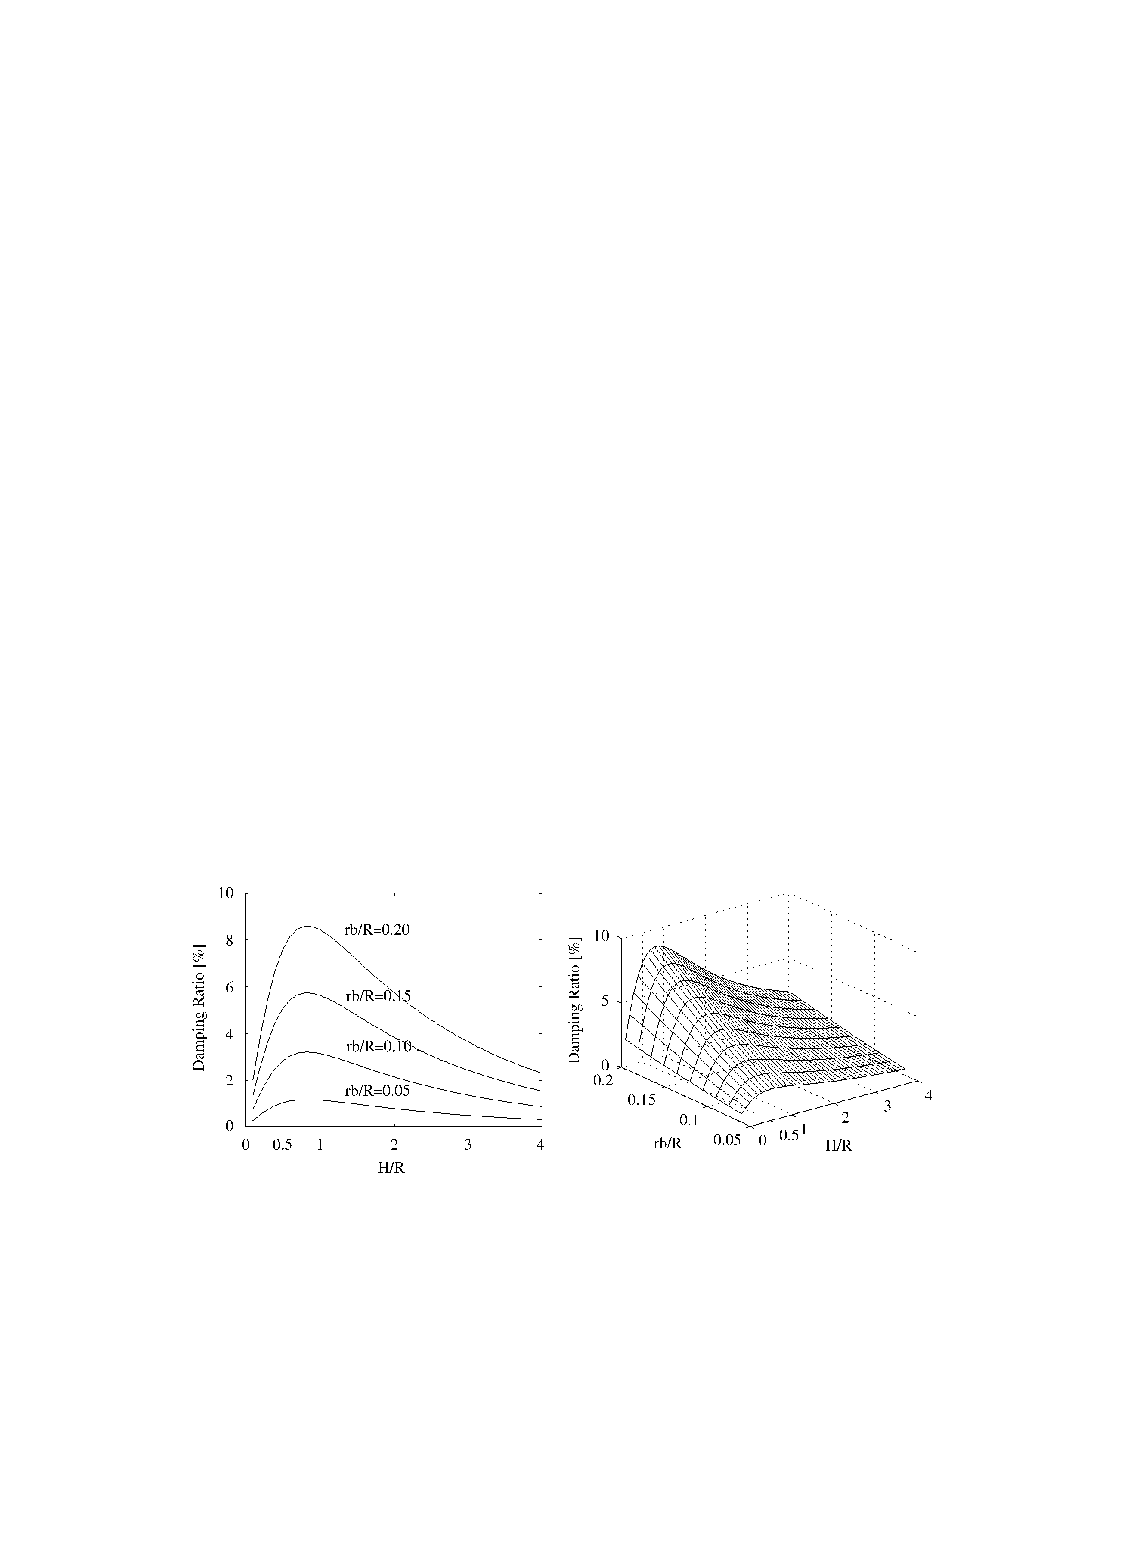
\includegraphics[width=\linewidth]{Ring-Baffle-Damping-Curve.pdf}
  \caption{有环形防晃板的贮箱液体阻尼}\label{Ring-Baffle-Damping-Curve}
\end{figure}

值得注意的是,由公式\eqref{eq:Ring-Baffle-Damping-Ratio}与Maleki的贮箱实验结果可以看出:液体阻尼将随液面高度$H/R$变化而变化;对于液体火箭来说,推进剂贮箱半满状态时的液体阻尼要远高于其满箱和空箱状态(如图\ref{Ring-Baffle-Damping-Curve}\cite{Maleki:2008},$\eta/R=0.05,\, r_b/R=0.2$)。此外,对于没有防晃板的情况而言,公式\eqref{eq:Empirical-Damping-Ratio}给出的计算结果不仅阻尼很小,并且没有体现这种变化趋势。这就要求POGO研究者们在对液体火箭带液贮箱进行建模分析的时候,必须格外关注以下几点:
\begin{enumerate}
	\item 严格区分不同类型贮箱的液体阻尼计算模型;
	\item 具备实验条件的情况下,尽可能开展带液贮箱的振动实验以验证计算结果的准确性;
	\item 必须考虑液体贮箱阻尼特性的时变规律。
\end{enumerate}

此外,随着近年来流体力学计算方法的发展,一些学者也开始尝试通过有限体积法的VOF方法对贮箱液体进行了更为精细的动态仿真。例如,杨魏等针对圆柱箱体中的液体晃动阻尼开展了数值仿真\cite{YangWei:2009},虽然其模型中应用的防晃板并非环形,但是贮箱内部液体的阻尼变化规律大致与Maleki模型相同(如图\ref{YangWei-Baffle},\ref{Damping-Ration-Yang})。鉴于液体火箭真实模型的贮箱实测非常难以实施,以上方法也为带液贮箱的阻尼特性分析提供了新的思路。

\begin{figure}[!htb]
\hspace{\stretch{2}}
\begin{minipage}[b]{0.35\textwidth}
  \centering
  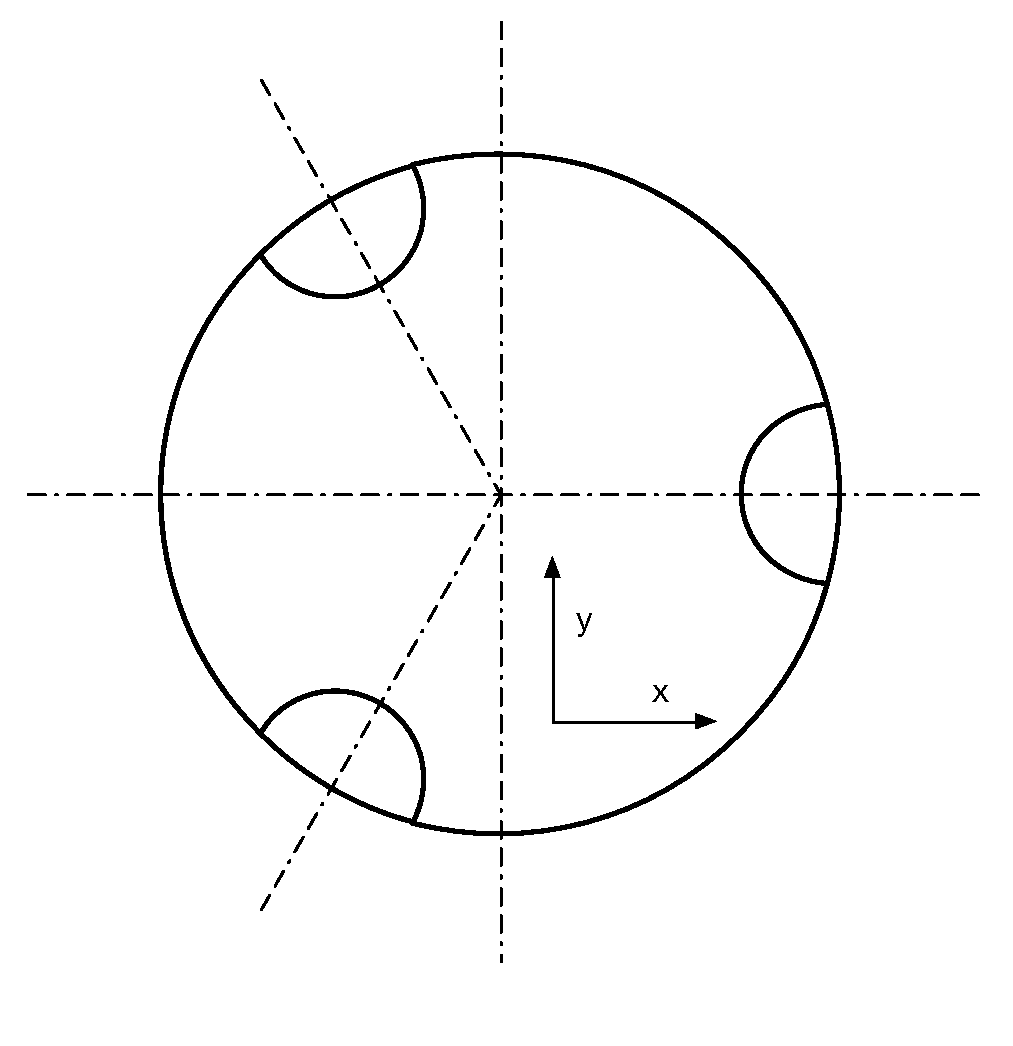
\includegraphics[width=\linewidth]{Baffle}
  \caption{半圆形防晃板配置图}\label{YangWei-Baffle}
\end{minipage}
\hspace{\stretch{1}}
\begin{minipage}[b]{0.55\textwidth}
  \centering
  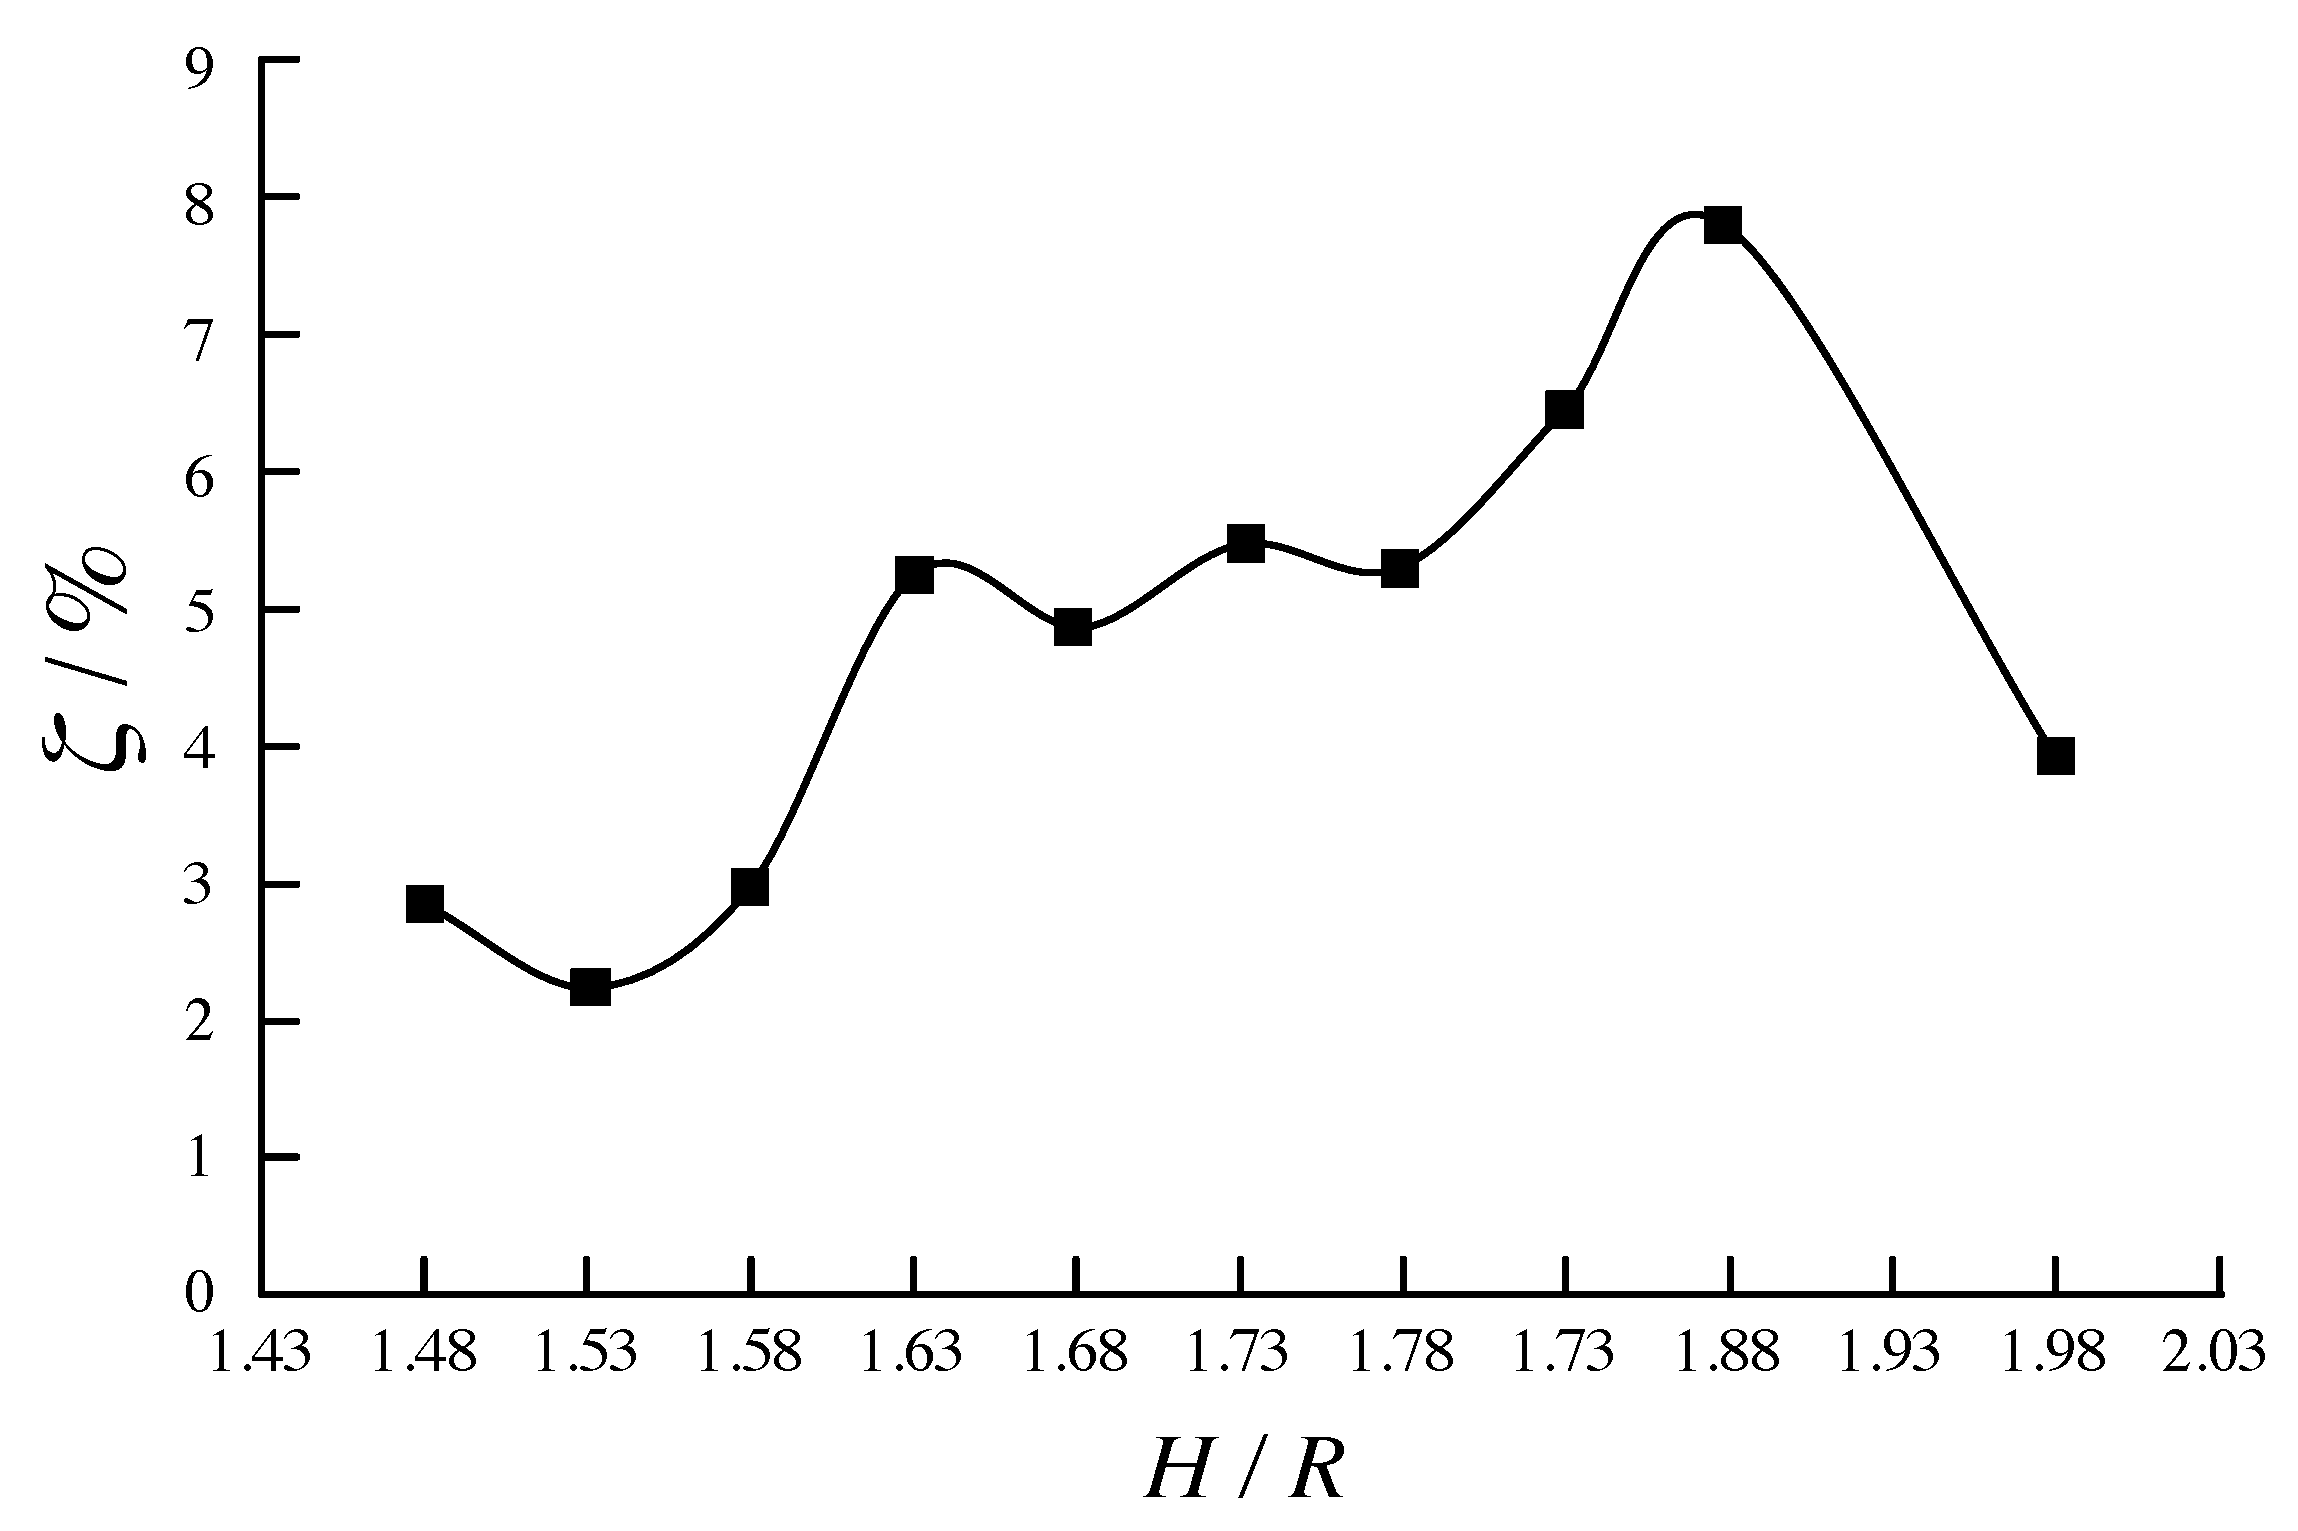
\includegraphics[width=\linewidth]{Damping-Ration-Yang}
  \caption{不同液面高度晃动阻尼比计算结果}\label{Damping-Ration-Yang}
\end{minipage}
\end{figure}

\subsection{贮箱液体阻尼的应用方法}
综合前两节的结论,可以看出耦合系统阻尼特性分析的重点和难点主要在于:
\begin{enumerate}[leftmargin=\parindent, align=parleft, labelindent=0pt, labelwidth=*]
\item 如何根据已有的带液贮箱实验数据及防晃板参数来确定阻力系数$C_d$,进而推导得出贮箱液体的阻尼比时变参数;
\item 如何将贮箱液体的阻尼特性包含于三维贮箱的建模之中,进而参与耦合系统动力学计算。
\end{enumerate}
由于前者的解决方法主要依赖现有实验手段而非进一步的理论推导,所以本节主要介绍如何在有限元方法中实现对于带液贮箱时变阻尼特性的建模分析。

在系统动力学中,阻尼通常可以分为粘性阻尼和结构阻尼两种,其数学描述如下:
\begin{equation}
	\begin{cases}
	f_v=b\dot{u} & \text{粘性阻尼力}\\
	f_s=\num{i}gku & \text{结构阻尼力} \\
	\end{cases}
\end{equation}
其中$\num{i}=\sqrt{-1}$,$b$为粘性阻尼系数,$g$为结构阻尼系数,$k$为结构刚度。可以看出,对于系统复模态分析来说,粘性阻尼力不仅与粘性阻尼系数相关,并且与外界扰动力频率$\omega$成正比。所以,若想通过调节阻尼系数来将两种阻尼模型等效互换,通常只能在特定频段之内操作:
\begin{equation}
	gk=b\omega\ \longrightarrow\ b=\frac{gk}{\omega}
\end{equation}
若外界扰动力频率$\omega$恰好等于系统固有频率,则
\begin{gather}
	\omega=\omega_n=\sqrt{\frac{k}{m}} \\
	b=\frac{gk}{\omega_n}=g\omega_n m
\end{gather}
由于系统的临界阻尼满足$b_c=2m\omega_n$,可以推导得出在共振点附近结构阻尼比$\zeta$满足:
\begin{equation}
	\label{eq:G-B-Zeta}
	\frac{b}{b_c}=\zeta=\frac{g}{2}
\end{equation}
假如已经通过实验等方法成功获取了带液贮箱的阻尼参数,可以根据公式\eqref{eq:G-B-Zeta}进行不同阻尼系数之间的换算。

系统复模态的计算方法通常可以分为两种:直接法和模态法。由于POGO振动的快速特征值求解法并没有采用模态缩聚技术,所以此处主要介绍如何针对直接法进行结构系统阻尼和贮箱液体阻尼的施加。

以MSC.Nastran为例,其阻尼输入方法可以分为两大类:直接矩阵输入法与参数设定法。
\begin{enumerate}[leftmargin=\parindent, align=parleft, labelindent=0pt, labelwidth=*]
\item 假如用户已经通过外部计算获得了系统阻尼矩阵,可以利用直接矩阵输入法将计算结果导入求解器(对称矩阵B2GG,对称或不对称矩阵B2PP);
\item 参数设定法则是通过指定模型中相关材料的结构阻尼系数$G_e$,或是直接设定系统整体的结构阻尼系数$G$或Rayleigh阻尼系数$\alpha_1,\alpha_2$\footnote{修改后的系统阻尼矩阵$\boldsymbol{B}'= \boldsymbol{B}+\alpha_1\boldsymbol{M}+\alpha_2\boldsymbol{K}$}来实现仿真对象的阻尼特性建模。
\end{enumerate}

\begin{figure}[!tb]
  \centering
  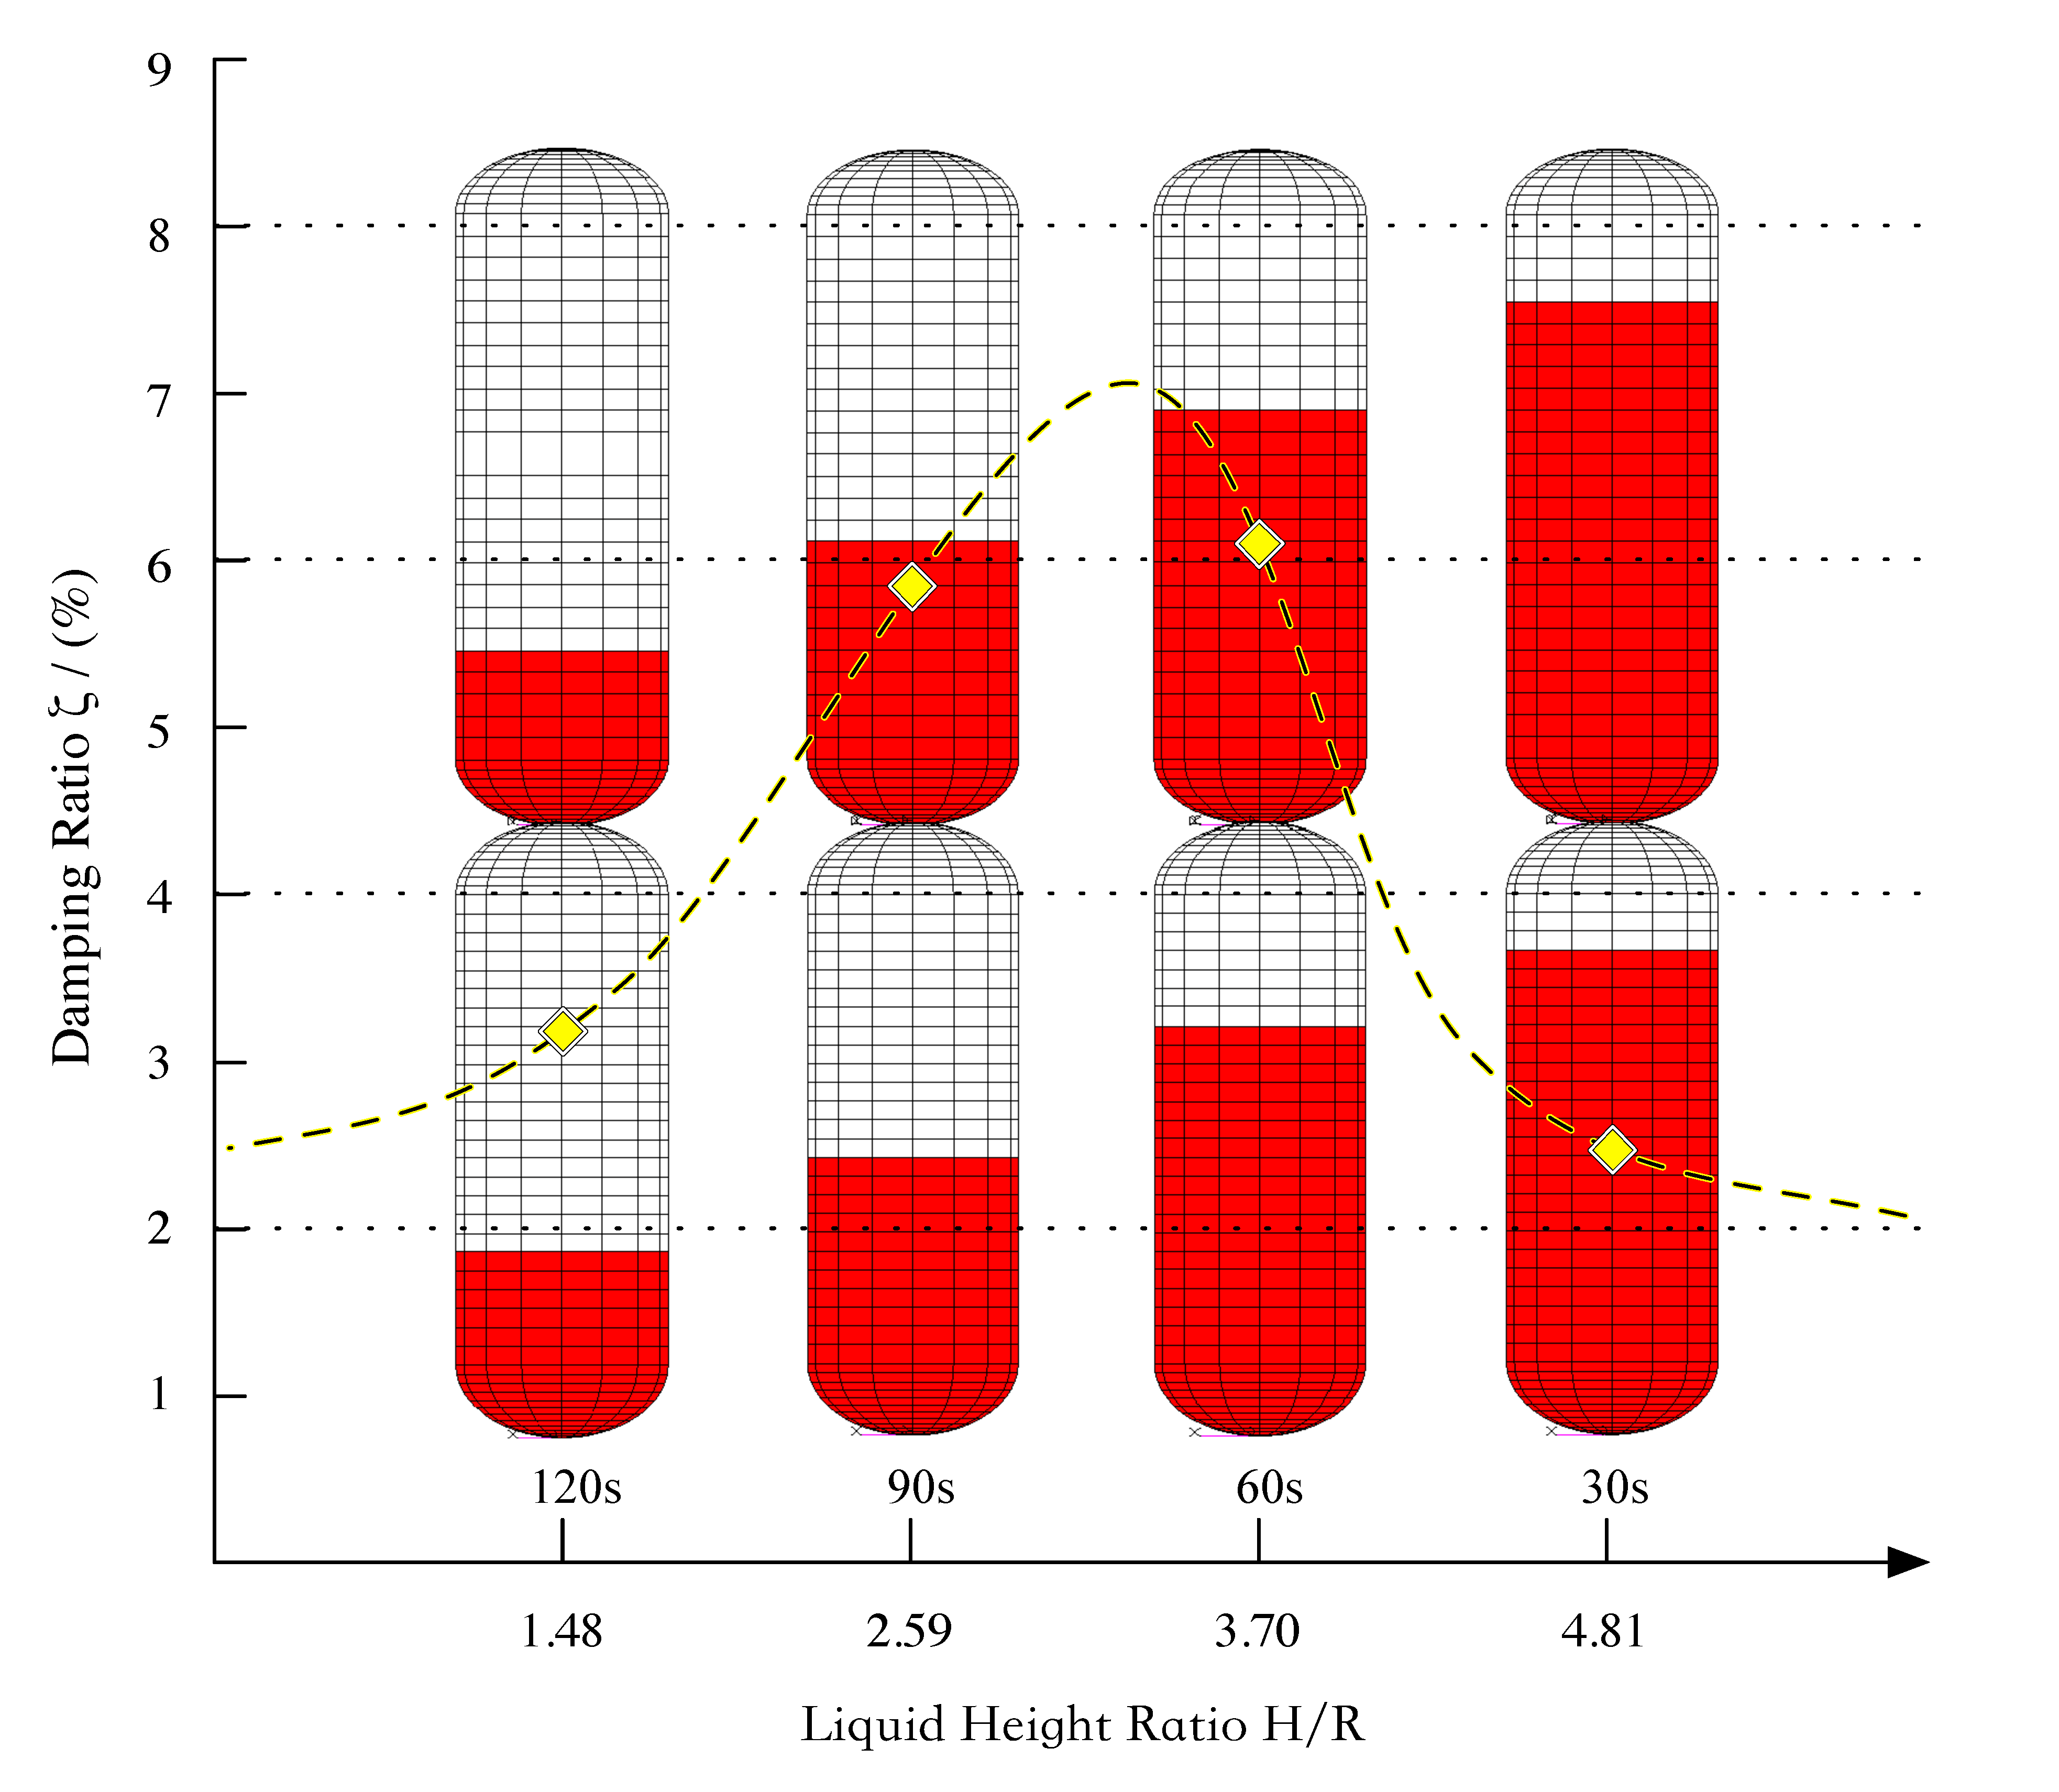
\includegraphics[width=\linewidth]{Time-Varing-Tank-Height}
  \caption{三维贮箱液体阻尼随高度变化示意图}\label{Time-Varing-Tank-Height}
\end{figure}

\section{算例分析}
参考节\ref{sec:Lumped-Numerical-Simulation}中算例,为了与其进行对比,本节采用同样的准静态技术与管路系统模型参数对相同规格的国内某液体火箭开展了耦合系统稳定性分析。不同的是,本例在对液体火箭结构系统建模时引入了节\ref{sec:3D-Liquid-Tank-Modelling}中介绍的带液贮箱三维模型,同时还利用节\ref{sec:3D-Tank-VS-Feedline-Update}中描述的TF卡建模方法对与其配套的管路系统进行对接处理。

\begin{figure}[p]
  \centering
  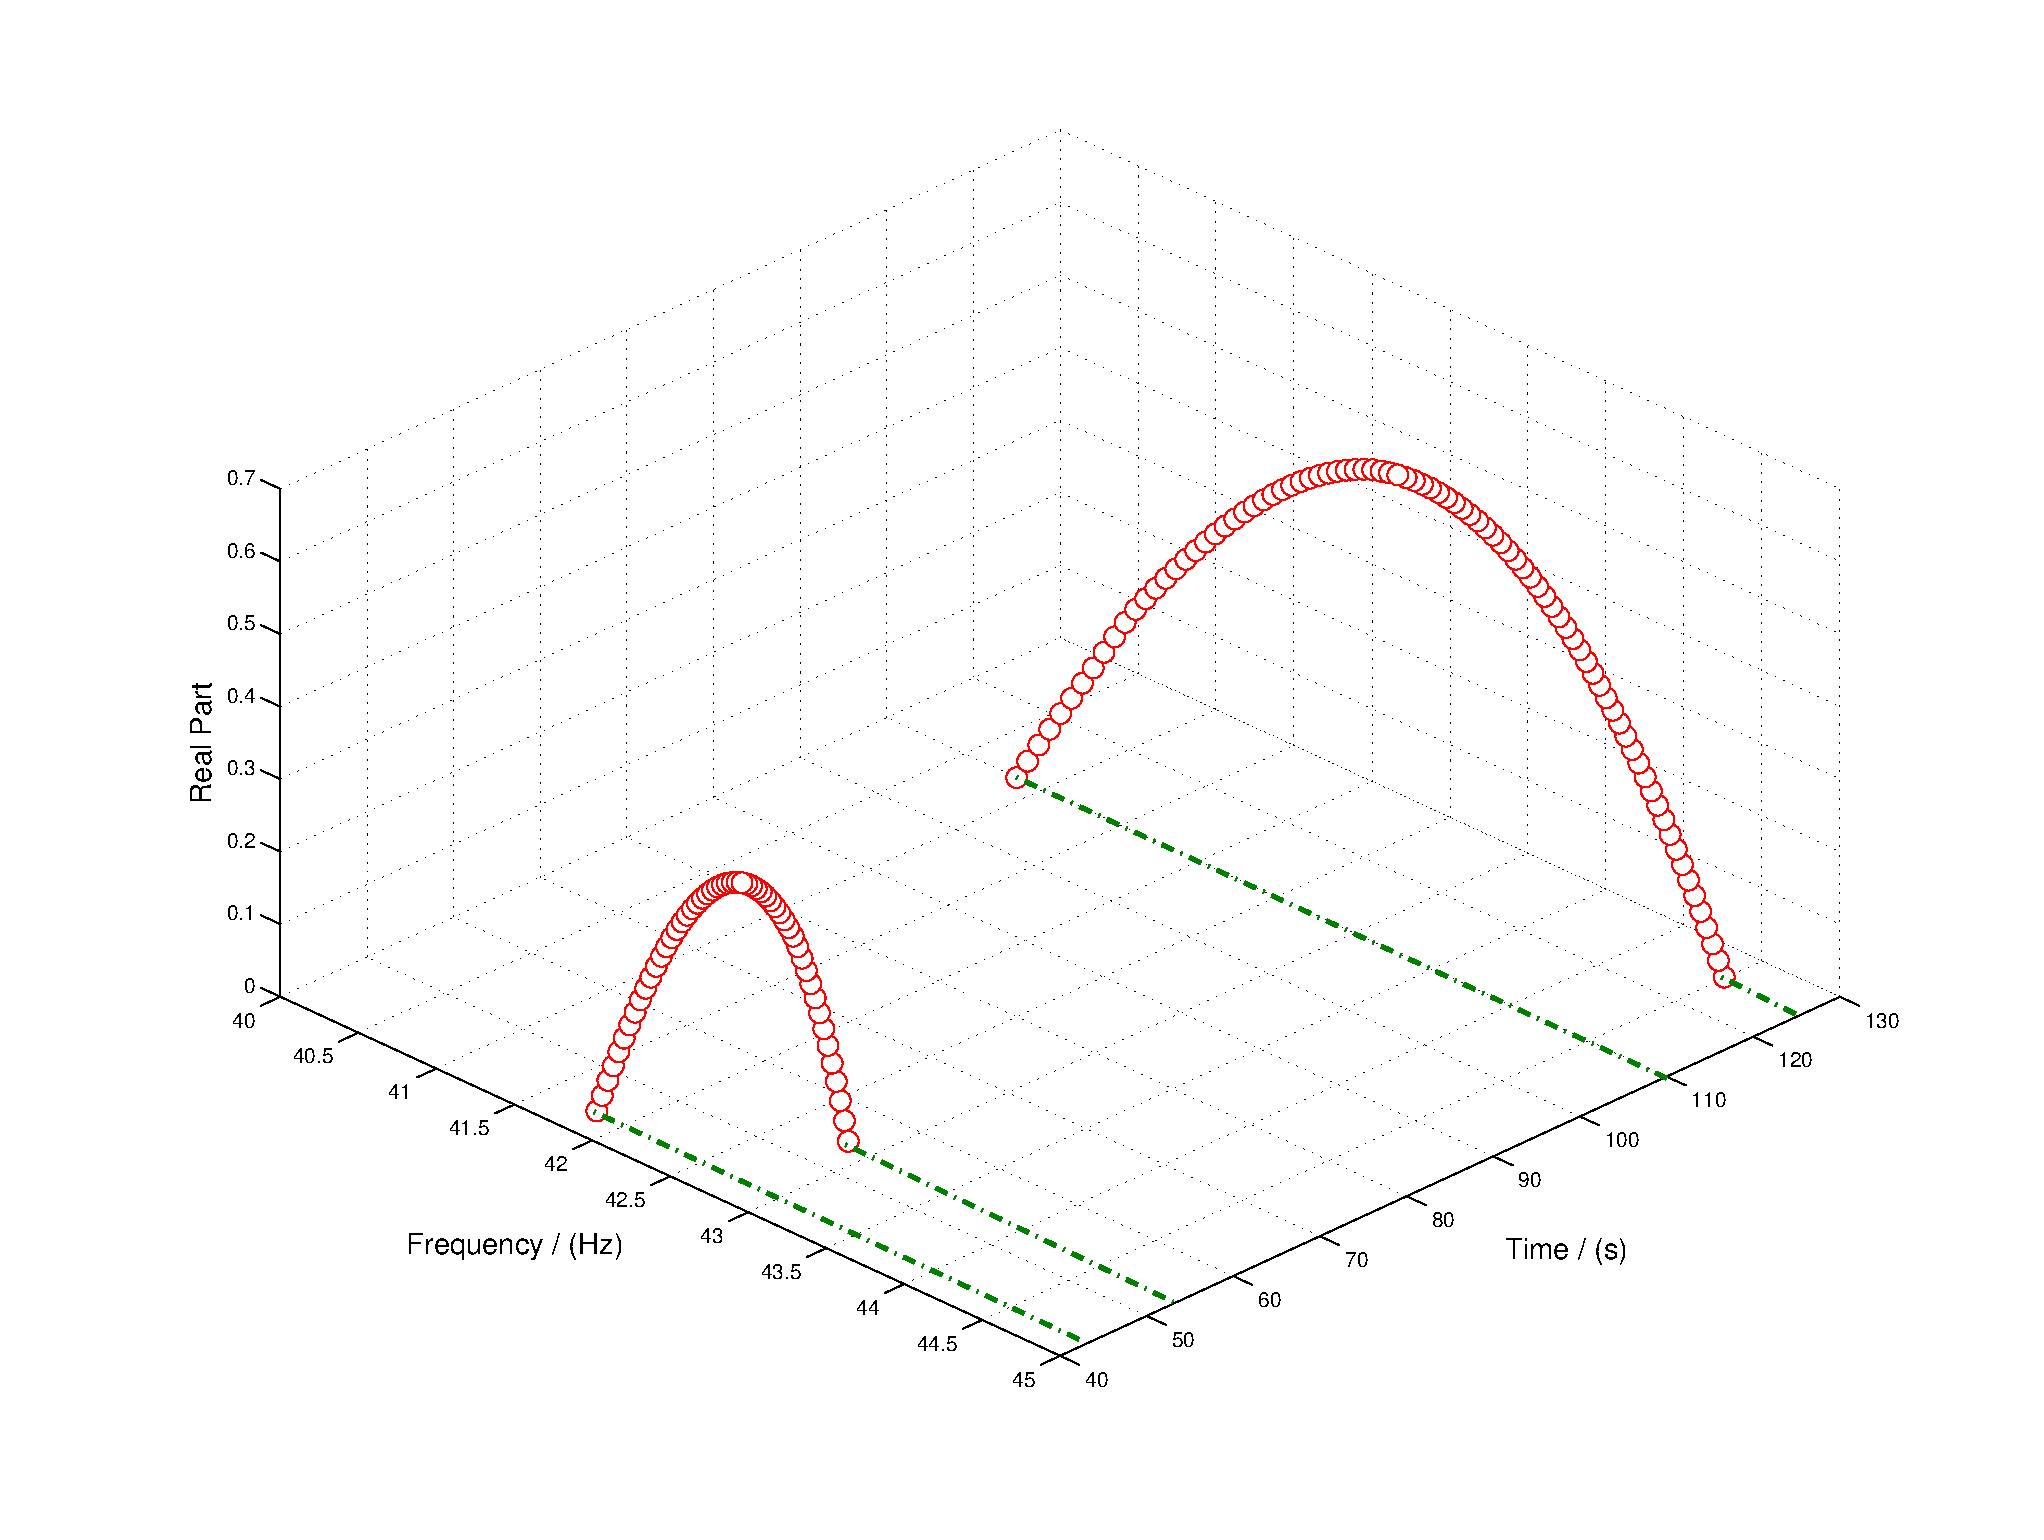
\includegraphics[width=\linewidth]{3D-Stability-Curve}
  \caption{耦合系统特征值随时间变化三维曲线}\label{3D-Stability-Curve}
  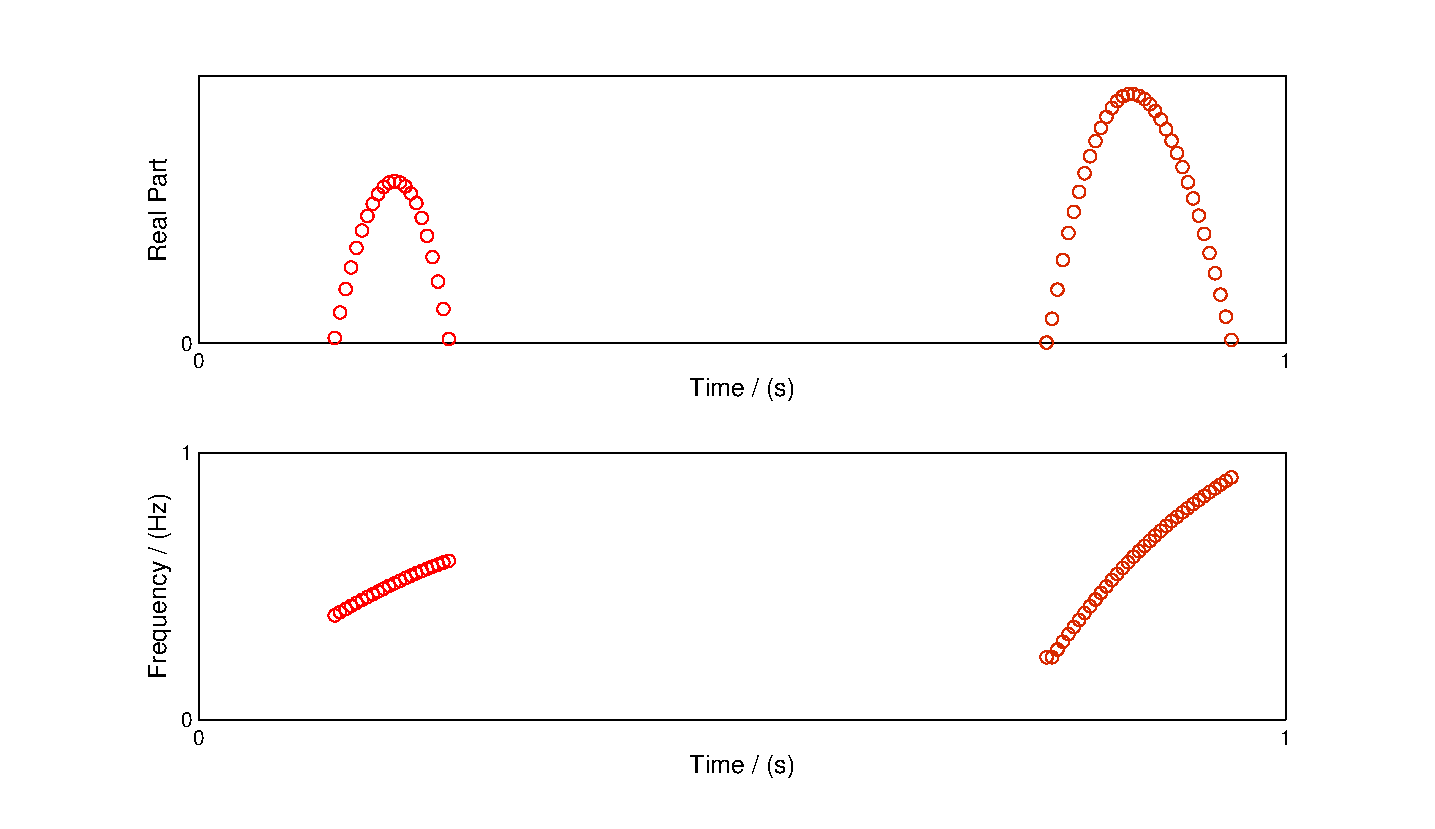
\includegraphics[width=\linewidth]{3D-Stability-Real-Imag}
  \caption{耦合系统特征值三维曲线的正视图与俯视图}\label{3D-Stability-Real-Imag}
\end{figure}

首先,图\ref{3D-Stability-Curve}给出了耦合系统特征值随时间变化三维曲线。由于POGO稳定性分析关注的主要为系统特征值是否包含正实部,所以图中仅显示了特征值包含正实部的部分结果。可以清晰的看出,相比与节\ref{sec:Lumped-Numerical-Simulation}中阐述的液体火箭为全时稳定的结论,该曲线表明此火箭在升空过程中经历了两个包含不稳定振动的时间区段。结合图\ref{3D-Stability-Real-Imag}给出的三维曲线正视图和俯视图,可以发现这两次不稳定振动存在以下特征:
\begin{enumerate}
	\item 不稳定模态的固有频率都随着时间从低到高变化;
	\item 不稳定模态的正实部时间演化都呈现抛物线形;
	\item 第二次失稳的时间历程与对应特征值的正实部较第一次来说更长、更大。
\end{enumerate}

从上述不稳定振动的特征描述来看,这两次失稳都基本符合POGO振动的主要特征。由于两次失稳的固有频率明显没有延续性,这就意味着该液体火箭不仅在运行期间发生了多次POGO振动,并且每次被激发的耦合系统模态可能不尽相同。

\setcounter{footnote}{0}
\begin{table}[tb]
	\renewcommand{\arraystretch}{1.5}
	\centering
	\caption{基于三维带液贮箱的耦合系统特征值}
	\label{table:3D-Rocket-EigenValue}
	\begin{tabular}{cccccc}
	\toprule
	\rule{8pt}{0ex}阶数\rule{8pt}{0ex} & 实部 & \rule{8pt}{0ex}频率(\si{\Hz})\rule{8pt}{0ex} & \rule{8pt}{0ex}阶数\rule{8pt}{0ex} & 实部 & \rule{8pt}{0ex} 频率(\si{\Hz})\rule{8pt}{0ex} \\ \midrule
	\textbf{1 } & $-$7.59E$-$01 & 8.47  & \textbf{16} & $-$2.59E$-$05 & 36.82 \\
	\textbf{2 } & $-$3.71E$-$01 & 8.86  & \textbf{17} & $-$2.74E$+$00 & 39.37 \\
	\textbf{3 } & $-$2.16E$+$02 & 10.07 & \textbf{18} & $-$8.46E$-$01 & 41.49 \\
	\textbf{4 } & $-$5.24E$-$01 & 10.64 & \textbf{19} & $-$6.49E$+$00 & 41.77 \\
	\textbf{5 } & $-$1.67E$-$06 & 16.32 & \textbf{20} & \framebox{\textcolor{red}{$+$2.99E$-$01}} & 42.73 \\
	\textbf{6 } & $-$1.05E$-$05 & 16.63 & \textbf{21} & $-$9.59E$+$00 & 47.73 \\
	\textbf{7 } & $-$9.90E$-$01 & 19.86 & \textbf{22} & $-$1.03E$+$01 & 49.03 \\
	\textbf{8 } & $-$1.54E$+$00 & 20.91 & \textbf{23} & $-$2.89E$-$04 & 49.69 \\
	\textbf{9 } & $-$2.03E$+$00 & 26.35 & \textbf{24} & $-$1.09E$+$01 & 50.22 \\
	\textbf{10} & $-$7.01E$-$01 & 28.56 & \textbf{25} & $-$2.53E$-$03 & 51.11 \\
	\textbf{11} & \framebox{\textcolor{red}{$+$1.21E$-$06}} & 29.66 & \textbf{26} & $-$2.25E$-$04 & 53.66 \\
	\textbf{12} & $-$8.44E$-$09 & 30.35 & \textbf{27} & $-$1.28E$+$01 & 54.52 \\
	\textbf{13} & $-$4.55E$+$00 & 32.67 & \textbf{28} & $-$1.98E$-$01 & 55.07 \\
	\textbf{14} & $-$1.13E$-$04 & 36.12 & \textbf{29} & $-$6.64E$+$00 & 56.62 \\
	\textbf{15} & $-$9.96E$-$06 & 36.66 & \textbf{30} & $-$1.60E$+$01 & 61.34 \\
	\bottomrule
	\end{tabular}
\end{table}

\begin{figure}[p]
  \centering
  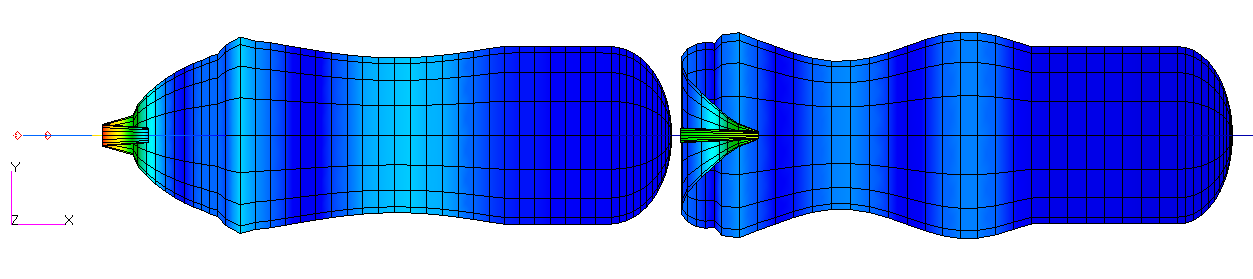
\includegraphics[width=\linewidth]{50s-Modal-Deformed.png}
  \caption{液体火箭带有正实部的贮箱局部模态剖面图:50s时刻}\label{50s-Modal-Deformed}
  \vspace{1.5em}
  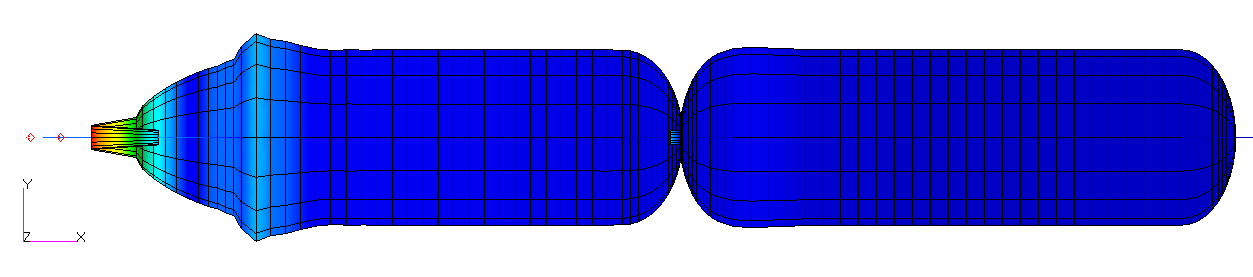
\includegraphics[width=\linewidth]{120s-Modal-Deformed.png}
  \caption{液体火箭带有正实部的贮箱局部模态剖面图:120s时刻}\label{120s-Modal-Deformed}
  \vspace{1.5em}
  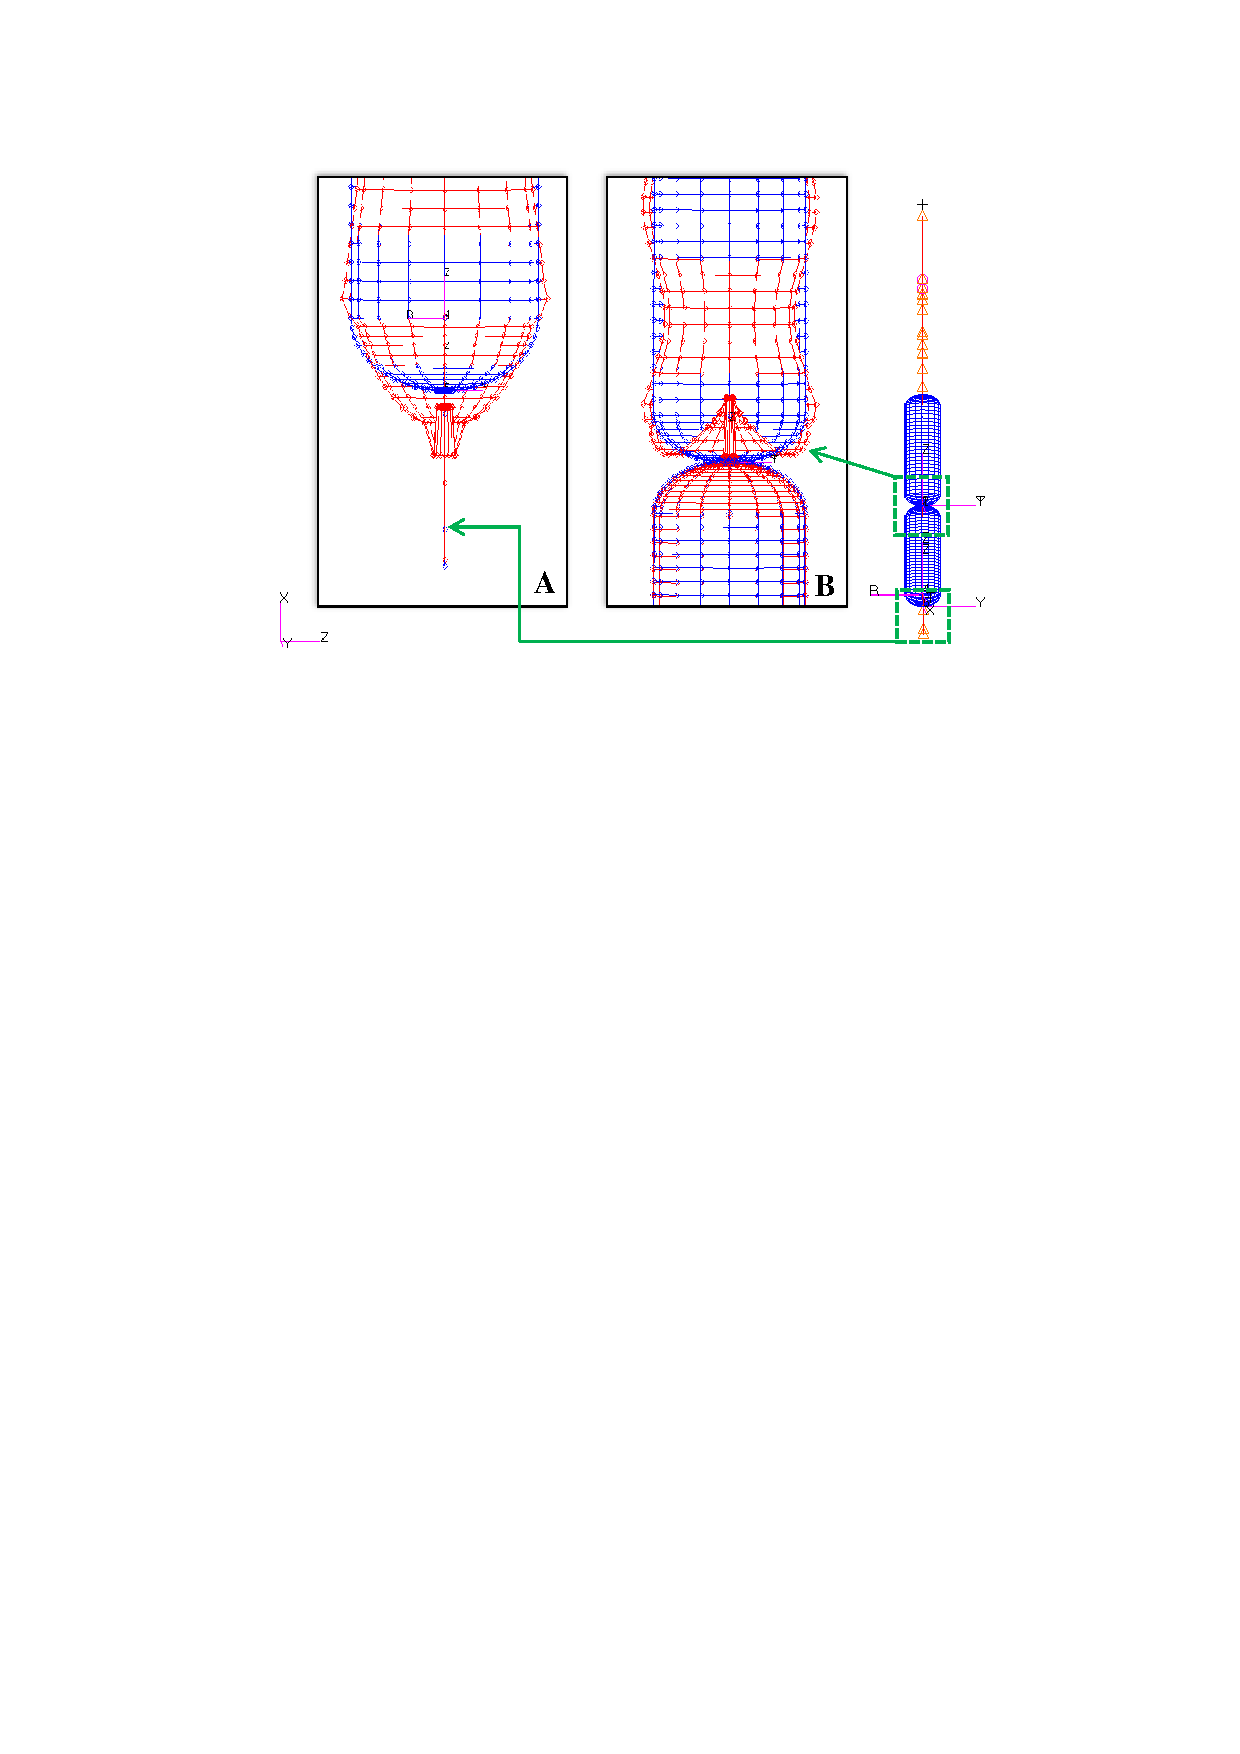
\includegraphics[width=\linewidth]{Deformed-Modal.pdf}
  \caption{液体火箭带有正实部的复模态局部振型:50s时刻}\label{Deformed-Modal}
\end{figure}

为了揭示POGO振动所处模态与其他正阻尼模态有何差异,图\ref{3D-Modal-Bottom}给出了两组耦合系统失稳模态与其相邻模态之间的局部振型形貌对比\footnote{各阶模态均采用统一的归一化方法}。通过观察氧化剂贮箱箱底及发动机燃烧室处的振动情况,可以发现:
\begin{itemize}
	\item[-] 由于推进剂贮箱壳体的柔度普遍高于液体火箭结构系统其他部位,所以耦合系统正阻尼模态通常也会展现出贮箱底部变形较大的情况;
	\item[-] 考虑到发动机燃烧室处的节点在质量和连接刚度上并无异于其他集中参数质量节点,所以其振动量级一般不会显著高于液体火箭其他部位。因此,在进行耦合系统复模态分析时,要特别关注在燃烧室处存在振动异常的高危振型---只有在发生POGO振动时,此处才有可能由于管路系统反馈力的影响而产生振幅剧烈放大的异常现象。
\end{itemize}







